
% \textbf{JEL codes:} P48, Q58, H23, Q54 % NCCcomment
% Q54 Climate • Natural Disasters and Their Management • Global Warming
% Q58 Government Policy (Q is Environmental econ)
% D78 Positive Analysis of Policy Formulation and Implementation
% H23 Externalities • Redistributive Effects • Environmental Taxes and Subsidies (H is public econ)
% P48 Political Economy • Legal Institutions • Property Rights • Natural Resources • Energy • Environment • Regional Studies (P4 is Other economic systems)
% H41 Public Goods
% H54 Infrastructures • Other Public Investment and Capital Stock

% \textbf{Keywords:} Climate change, global policies, cap-and-trade, attitudes, survey.%, inequality, wealth tax. % NCCcomment

\tableofcontents

\onehalfspacing % NCCcomment

%\clearpage
\begin{bibunit}

\section{Introduction}% NCCcomment
% TODO!? Now at 62? 
% Inequality between countries: https://data.worldbank.org/indicator/NY.GDP.PCAP.PP.CD?contextual=default&end=2021&locations=EU-ZG-XD-XM-1W-IN-US-CD-BI-LU-CN&start=2021&view=bar (PPP current $) / https://data.worldbank.org/indicator/NY.GDP.PCAP.CD?end=2021&locations=EU-ZG-XD-XM-1W-IN-US-CD-BI-LU-CN&start=2021&view=bar (current $) / https://data.worldbank.org/indicator/NY.GDP.PCAP.PP.KD?end=2021&locations=EU-ZG-XD-XM-1W-IN-US-CD-BI-LU-CN&start=2021&view=bar (PPP 2017 $) / Pop high-income 1.2G, low-income 700M https://data.worldbank.org/indicator/SP.POP.TOTL?locations=XD-XM

% TD change the intro, e.g. Global poverty and climate change are among the most critical issues faced by the world today", and then explain that the first could be solved by transfer, the second by capping pollution, hence an effective policy to tackle these two problems is the GCS. Yet, this policy is nowhere to be seen in policy debates. Why? In this paper we provide evidence from surveys showing that people all over the world support this policy. To explain this paradox (people stated support vs absence of the policy), we further investigate the sincerity of these claims and rationales behind the support, etc.

Major sustainability objectives could be achieved by global approaches to mitigating climate change and poverty involving transfers from high- to lower-income countries.\citep{budolfson_climate_2021,franks_mobilizing_2018,dennig_inequality_2015,soergel_combining_2021,bauer_quantification_2020,cramton_global_2017} 
For instance, a global wealth tax could finance the Sustainable Development Goals.\citep{piketty_brief_2022} More specifically, if merely 35\% of the revenue were allocated for this purpose, a global 2\% tax on individual wealth in excess of \$5 million could significantly reduce poverty as it would mechanically increase low-income countries' national income by 50\% (as computed on the \href{https://wid.world/world-wealth-tax-simulator/}{WID wealth tax simulator}). 
Besides, global carbon pricing is widely regarded by economists as the benchmark climate policy, as it would efficiently correct the carbon emissions externality. As early as 1990, Michael Grubb stated:\cite{grubb_greenhouse_1990} ``by far the best combination of long term effectiveness, feasibility, equity, and simplicity, is obtained from a system based upon tradable permits for carbon emissions which are allocated on an adult per capita basis'', i.e., equally among human adults. Support for such solution, which we call the ``Global Climate Scheme'', has been renewed ever since.\citep{hoel_carbon_1991,agarwal_global_1991,bertram_tradeable_1992,baer_equity_2000,jamieson_climate_2001,blanchard_major_2021} % rajan_global_2021

While international negotiations have not yet led to ambitious globally redistributive policies, recent developments suggest that such a change might be underway. The %International Maritime Organization is poised to adopt a global carbon levy on maritime fuel; the 
African Union \href{https://media.africaclimatesummit.org/NAIROBI+Declaration+FURTHER+edited+060923+EN+920AM.pdf}{calls for} a global carbon taxation regime, %\cite{african_union_african_2023} 
the UN \href{https://digitallibrary.un.org/record/4032838}{is setting up} a Framework Convention on International Tax Cooperation, %\cite{un_promotion_2023} 
% Brazil uses its presidency of the G20 in 2024 to propose 
the G20 is studying 
a global wealth tax, % https://www.climatechangenews.com/2024/04/19/global-billionaires-tax-to-fight-climate-change-and-hunger-rises-up-political-agenda/
% \href{https://www.lemonde.fr/idees/article/2023/03/14/taxation-mondiale-sur-les-ultrariches-ce-que-nous-avons-reussi-pour-les-multinationales-nous-devons-le-faire-pour-les-grandes-fortunes_6165354_3232.html}{backed} by 130 Members of the European Parliament; 
etc. 

A key condition for implementing global policies has remained largely unaddressed: the support of citizens. Using a Global survey on 40,680 respondents from 20 high- and middle-income countries, we reveal substantial support for those policies, especially global climate policies and a global tax on the wealthiest aimed at financing low-income countries (other questions from this survey are analyzed in a companion paper\cite{dechezlepretre_fighting_nodate}). Interestingly, even in wealthy nations that would bear a significant burden, majorities of citizens express support for such globally redistributive policies. To better understand public support for global policies in high-income countries, we conduct our Main surveys among 8,000 respondents from France, Germany, Spain, the UK, and the U.S. 

% By studying in depth the support for global policies, we are making an ambitious shift in the methodological approach of attitudinal surveys. In general, academic surveys focus on studying effect sizes of some treatment on political attitudes, or the socio-demographic factors that correlate with attitudes.\cite{kuziemko_how_2015,douenne_yellow_2022} The magnitude of support for a given proposal is often regarded as problematic to estimate satisfactorily. %unsuitable for satisfactory estimation. 
% The measure of support is usually left to non-academic pollsters, who rarely apply all the academic best practices: transparency, representative sampling, neutral and precise wording of questions, comparison with existing literature, use of multiple questions and complementary methods to correctly interpret the results. Although estimating the extent of support is challenging, this question seems too important not to be addressed using scientific methods. Absent large scale measurements of public opinion like referenda, surveys remain the best method to assess support or opposition to given policies. In this paper, after a worldwide assessment in the Global survey, we use our Main surveys to carefully measure the support for global policies in Western countries. We inquire the support for various policies, approach the question from diverse angles, and run a battery of pre-registered tests to check whether stated support estimates are reliable.

The focus of the Main surveys is a specific policy aimed at addressing both climate change and poverty, referred to as the ``Global Climate Scheme'' (GCS). It implements a cap on carbon emissions to limit global warming below 2\textdegree{}C. The emission rights are auctioned each year to polluting firms and fund a global basic income, alleviating extreme poverty. 
This archetypal policy exposes respondents to the key trade-off between the benefits and costs of globally redistributive climate policies, as respondents are made aware of the cost that the GCS entails for their country's people. 

After checking that respondents have understood the policy and its cost, we measure the support in a direct \textit{Yes}/\textit{No} question. The GCS is supported by three quarters of Europeans and more than half of Americans. Then, we test for social desirability bias using a list experiment. We find no evidence that people exaggerate their support in the direct question. To assess whether the support would diminish in a context with real stakes, we ask respondents whether they are willing to sign a petition in favor of the GCS, after informing them that the question results will be communicated to their head of state's office. The support is sustained in an environment that approaches real stakes. We then carry out conjoint analyses to neutralize experimenter demand and investigate the priority given to global policies compared to other types of policies. Conjoint analyses reveal that a political platform is more likely to be preferred if it contains the GCS or a global tax on millionaires, and that global policies rank high in the prioritization of policies. Our randomized experiments also show that a candidate would not lose vote intentions by endorsing the GCS, and might even gain up to 11 points in a country like France. An analysis of open-ended fields confirms that support for the GCS is real, and indicates that appeal of the GCS comes from its international nature and its impacts on climate, more than on global poverty. % from addressing climate change at the international level, more than alleviating poverty. 
We also test other global policies and universalistic attitudes. Support is very strong for a global tax on millionaires, and the median respondent prefers to allocate 30\% of the revenues of such a tax to low-income countries. Majorities are willing to increase foreign aid, but only if some conditions are respected, such as making sure the aid is well spent and other high-income countries also increase their contribution. Questions on universalistic values, including a donation experiment, confirm the congruence of underlying values with the support for specific policies. Our diverse approaches also help understand what drives the support. For instance, the evidence indicates that one key reason why increasing foreign aid is not as popular as global policies lies in its unilateral nature.
% We reckon that survey evidence is no panacea, as attitudes can be ambivalent and context-dependent. Nevertheless, we arguably employ the best available methods to address potential concerns, including an experiment assessing how support might be affected by a negative media campaign. 

Overall, our results %  consistently 
point out to strong and genuine support for global climate and redistributive policies, as our experiments confirm the stated support found in direct questions. 
% This suggests that carefully administered surveys can be used to measure the level of support for a given policy. 
Our results contribute to the literature on attitudes toward climate policy, confirming that climate policy is preferred at a global level,\citep{issp_international_2010,beiser-mcgrath_could_2019,sivonen_attitudes_2022,meilland_international_2023} where it is more effective and fair. 
While 3,354 economists supported a national carbon tax financing equal cash transfers in the \href{https://www.clcouncil.org/media/EconomistsStatement.pdf}{Wall Street Journal}, numerous surveys have shown that support for such policy is mixed at best.\citep{douenne_yellow_2022,dechezlepretre_fighting_nodate,carattini_overcoming_2018,maestre-andres_perceived_2019,mildenberger_limited_2022} Meanwhile, the GCS --- the global version of this policy --- is largely supported, despite higher costs in high-income countries. 
% Indeed, the Global Climate Scheme is largely supported, but a similar policy at the national level is opposed by a majority in many countries,\citep{dechezlepretre_fighting_nodate} despite lower costs. 
% Noting that only 13\% of French people declared supporting a national carbon tax with cash transfers during the Yellow Vests movement,\citep{douenne_yellow_2022} surveys appear to accurately reflect the level of support. Therefore, unless support for global policies disappear once they enter the public debate, it seems unlikely that a policy such as the GCS would face major protests. % TODO? cut?
In our discussion we offer potential explanations behind the lack of prominence of global policies in the public debate despite this strong support. 
% Finally, while our findings underscore majority support for global policies, converging results from independent surveys are needed to ascertain such novel evidence. %, even in the absence of significant policy proposal. 

%%%%%%%%%%%%%%
% Major sustainability objectives could be achieved by global approaches to mitigating climate change and poverty involving transfers from high- to lower-income countries \citep{budolfson_climate_2021,franks_mobilizing_2018,dennig_inequality_2015,soergel_combining_2021,bauer_quantification_2020,cramton_global_2017}. 
% Yet international negotiations have not led to ambitious globally redistributive policies. 
% We examine a key condition for achieving sustainability objectives: the support of citizens for such global policies. %This article investigates public attitudes towards such global policies.

% Recent surveys administered to 40,680 respondents from 20 high- and middle-income countries reveal substantial support for those policies, especially global climate policies and a global tax on the wealthiest aimed at financing low-income countries (other questions from these surveys are analyzed in a companion paper, \citealp{dechezlepretre_fighting_nodate}). In particular, a global 2\% tax on individual wealth in excess of \$5 million would effectively reduce poverty as it would mechanically increase low-income countries' national income by 50\%, if merely 35\% of the revenue were allocated for this purpose.\footnote{Figures derived from \citet{chancel_world_2022}, the \href{https://wid.world/world-wealth-tax-simulator/}{WID wealth tax simulator}, and the World Bank.} Interestingly, even in wealthy nations that would bear a significant burden, majorities of citizens express support for such globally redistributive policies.% I have added the following lines. TODO? put in a footnote?
% % Using the price and emissions trajectories from the report by \cite{stern_report_2017}, %Stern-Stiglitz report,\cite{stern_report_2017} 
% % we estimate that the basic income would amount to \$30 per month for each human above 15 in 2030, enough to lift out of extreme poverty the 700 million people who live with less than PPP \$2 per day. Conversely, assuming a carbon price of \$90/tCO$_\text{2}$ in 2030, high emitters like a typical American (with median U.S. CO$_\text{2}$ emissions) would lose in net \$85 per month, as they would face \$115 per month in price increases (see details in Appendix \ref{app:gain_gcs}). 


% To gain insights into the factors shaping public support for global policies in high-income countries, we conduct complementary surveys among 8,000 respondents from France, Germany, Spain, the U.S., and the UK. The focus of our approach is a specific policy aimed at addressing both climate change and poverty, referred to as the ``Global Climate Scheme'' (GCS). It implements a cap on carbon emissions to limit global warming below 2\textdegree{}C. The emission rights are auctioned each year to polluting firms and fund a global basic income, alleviating extreme poverty.\footnote{Although the GCS may seem idealistic, we focus on this policy as its key features allow us to expose respondents in a concise and simple way with the key trade-off between the costs and benefits of globally redistributive climate policies.} 
% In the wording of the question, respondents are made aware of the cost to themselves of such global redistribution. 
% The GCS is supported by three quarters of Europeans and half of Americans. We test whether support of the expressed preference is sincere: a list experiment shows no evidence of social desirability bias in survey responses, majorities are willing to sign a real-stake petition (with the question results communicated to the heads of state), and global redistribution ranks high in the prioritization of policies. Conjoint analyses reveal that a political platform is more likely to be preferred if it contains the GCS or a global tax on millionaires. 
% Besides, we uncover strong stated support for other globally redistributive policies such as increased foreign aid or the democratization of global institutions, and most respondents express some degree of universalism in their underlying values. 
% % By employing a list experiment, a real-stake petition (with the question results communicated to the heads of state), 
% % and conjoint analyses, our study indicates genuine and robust support for the GCS among respondents. For example, the conjoint analyses provide evidence that political parties would not lose vote intention by endorsing the GCS.% https://data.worldbank.org/indicator/NY.GDP.MKTP.CD?locations=XD-XM

% % On top of addressing both global poverty and climate change, we provide evidence from surveys showing that people all over the world support this policy. Yet, the GCS is nowhere to be seen in policy debates. Why? To explain this paradox (absence of the policy despite majority stated support), we further investigate rationales behind the support for the GCS and the sincerity of these claims, as well as attitudes toward other global policies, global redistribution, and universalistic values. % TODO: rework

% These findings underscore a strong and genuine support for global climate and redistributive policies. %, even in the absence of significant policy proposal. 
% In our discussion we offer potential explanations behind the lack of prominence of global policies in the public debate despite this strong support. %policy implementation gap.


% Global cooperation is necessary to solve sustainability challenges such as poverty and climate change. Disagreements on burden-sharing, differing priorities and lack of institutional capacity are obstacles to effective global collaboration. One further obstacle, neglected in social science research so far, is the willingness of citizens in affluent countries to bear the costs of the global redistribution associated with effective poverty reduction and climate change mitigation. This article investigates public attitudes towards global policies delivering on climate change mitigation and poverty reduction.

% To explore relevant public attitudes, we use surveys administered to over 40,000 respondents from 20 high- and middle-income countries covering 72\% of global carbon emissions. The responses reveal substantial support for global policies, including global emissions trading and a global wealth tax aimed at financing low-income countries. Surprisingly, even in wealthy nations that would bear a significant burden, majorities of citizens express support for globally redistributive measures.

% To gain insights into the factors shaping public support in these countries, we conducted complementary surveys among 8,000 respondents from France, Germany, Spain, the U.S., and the UK. The focus is a specific policy aimed at addressing both climate change and extreme poverty, referred to as the ``Global Climate Scheme'' (GCS). It consists of global emissions trading, which limits total carbon emissions. The emission rights are auctioned each year to polluting firms and fund a global basic income. By employing a list experiment, a real-stake petition, and conjoint analysis, our study demonstrates the genuine and robust support for the GCS among respondents. For example, the conjoint analysis provides evidence that policymakers do not lose public support by endorsing the GCS.

% These findings underscore a strong demand for globally redistributive climate policies, even in the absence of significant policy implementation. In our discussion we offer potential explanations behind this policy implementation gap.


% Ethical theories often warrant transfers from high- to low-income people, hence from high- to low-income countries. This is the case of utilitarianism, the benchmark ethical theory used in economics. Utilitarianism assigns the same weight to each person and thus considers that a dollar is better allocated to a low-income person, which has a higher marginal utility than a high-income person.\cite{mill_utilitarianism_1861} 

% Addressing global poverty, inequalities and climate change are at the heart of the universally agreed Sustainable Development Goals (SDG). % 12 out of  17
% It has been pointed out that low-income countries generally do not have enough domestic resources to eliminate the poverty gap in the short run.\cite{bolch_arithmetics_2022} % In other words, it would hardly be possible to achieve the first SDG and end extreme poverty by 2030 without international transfers. => Careful, Bolch use a poverty line above the SDG one.

% Climate change is another issue that calls for a global response and in particular international transfers. Postulating %Assuming
% that each human has an equal right to emit CO$_\text{2}$, low emitters have a legitimate claim \textit{vis-à-vis} high emitters, that can be settled by monetary transfers. Coupling this burden-sharing principle to the carbon budget (remaining emissions that would be compatible with the Paris agreement) naturally defines a global climate policy. We call it the ``Global climate scheme'' (GCS); it consists of a global cap-and-trade system where emission rights are auctioned each year to polluting firms and the revenues finance a global basic income. Using the price and emissions trajectories from the Stern-Stiglitz report,\cite{stern_report_2017} we estimate that the basic income would amount to \$30 per month for each human above 15 in 2030, enough to lift out of extreme poverty the 700 million people who live with less than PPP \$2 per day. Conversely, high emitters like a typical American (with median U.S. CO$_\text{2}$ emissions) would lose in net \$85 per month, as they would face \$115 per month in price increases (assuming a carbon price of \$90/tCO$_\text{2}$ in 2030). % TD Give the numbers in the Results section
% % G default policy for economists, we focus on it; transfers at heart of COP; global wealth tax proposed by Piketty, Saez (fair and effective); democratisation of int'l institutions recurring topic.
% % Few studies on CC burden-sharing, all compatible with G
% % Few studies on global policies, but they show support (Ghassim, Carattini 19)
% % Here, two sets of results. First, twenty countries. Second, dig deeper using complementary survey.

% If high emitters share universalistic ethical values, we expect strong support for the GCS, even in high-income countries. On the contrary, if people defend their own financial interest, we expect low support for the GCS in high-income countries. 

% In this paper, we study attitudes toward global policies that address climate change, global poverty or inequalities, with a focus on the GCS. We measure stated support for different global policies using unpublished results from a survey\cite{dechezlepretre_fighting_nodate} on climate attitudes conducted in 2021 on 40,680 respondents from 20 countries covering 72\% of global CO$_\text{2}$ emissions. We then conduct a representative survey on 3,000 U.S. respondents to study in detail the sincerity and rationales behind the support for the GCS, the attitudes toward various global policies, global redistribution, and universalistic values.

\paragraph{Literature} 
% Although international surveys have shown widespread support for costly climate action \citep{dechezlepretre_fighting_nodate,leiserowitz_international_2022,andre_globally_2024}, few prior attitudinal surveys have examined policies for global redistribution. Exceptions include \citet{carattini_how_2019}, who study global carbon taxes with international per capita redistribution and find agreement close to 50\% in high-income countries. % TODO?  (but do not examine an emissions cap nor the sincerity of support)
% In addition, \citet{issp_international_2019} uncover near consensus that ``present economic differences between rich and poor countries are too large'' (overall, 78\% agree and 5\% disagree) in each of 29 countries. \citet{fehr_your_2022} show that, contrary to national redistribution, support for global redistribution does not depend on one's income relative to its fellow citizens but on its country's income per capita. \citet{ghassim_public_2022} examine support for global democracy in a range of countries and finds that, in countries governed by a coalition, voting shares would shift by 8 (Brazil) to 12 p.p. (Germany) from parties that are said to oppose global democracy to parties that supposedly support it. Appendix \ref{sec:literature} contains a broader literature review including further attitudinal surveys on global policies (\ref{subsubsec:literature_attitudes_policies}); prior work on attitudes toward climate burden sharing (Appendix \ref{subsubsec:literature_attitudes_burden_sharing}), attitudes toward foreign aid (Appendix \ref{subsubsec:literature_foreign_aid}); global carbon pricing (Appendix \ref{subsubsec:literature_pricing}), global redistribution (Appendix \ref{subsubsec:literature_redistribution}), basic income (Appendix \ref{subsubsec:literature_basic_income}), and global democracy (Appendix \ref{subsubsec:literature_democracy}).
% TODO? Furthermore, correcting misperceptions concerning one's position in the world's income distribution does not affect the support for global redistributive policies.\cite{fehr_your_2022}

International surveys have shown widespread support for costly climate action.\citep{dechezlepretre_fighting_nodate,leiserowitz_international_2022} For instance, representative surveys in 125 countries covering 96\% of the world's greenhouse gas emissions show that 69\% of the global population express willingness to contribute 1\% of their income to fight global warming.\cite{andre_globally_2024} International surveys have also uncovered near consensus that ``present economic differences between rich and poor countries are too large'' (overall, 78\% agree and 5\% disagree) in each of 29 countries.\citep{issp_international_2019} 

Yet, few prior attitudinal surveys have examined global redistributive policies. 
A notable exception tests the support for six variants of a global carbon tax on samples in five countries, representative along gender and age.\cite{carattini_how_2019} For a given variant, the sample size is about 167 respondents per country. They find over 80\% support for any variant in India, between 50\% and 65\% in Australia, the UK and South Africa, and 43\% to 59\% in the U.S., depending on the variant. Notably, the support for a global carbon tax funding an equal cash transfer for each human is close to 50\% in high-income countries (e.g., at 44\% in the U.S.). These figures are consistent with our results from the \textit{Global} survey (see Figure \ref{fig:oecd}), where the support is lower for a tax that would ``only'' reduce CO$_\text{2}$ emissions than for a quota that would unambiguously achieve the climate target. 
Relatedly, 66\% of Americans support providing ``financial aid and technical support to developing countries that agree to limit their greenhouse gas emissions'';\cite{leiserowitz_public_2021} and 90\% of Germans want some degree of global redistribution.\cite{fehr_your_2022} 
Besides, in surveys conducted in Brazil, Germany, Japan, the UK and the U.S., support ranges from 55\% to 74\% for ``a global democracy including both a global government and a global parliament, directly elected by the world population, to recommend and implement policies on global issues''.\cite{ghassim_who_2020} % (for example, international peace, world poverty, and climate change)''
Through an experiment, this paper also finds that, in countries where the government stems from a coalition, voting shares would shift by 8 (Brazil) to 12 p.p. (Germany) from parties who are said to oppose global democracy to parties that supposedly support it. For instance, when Germans respondents were told that (only) the Greens and the Left support global democracy, these parties gained respectively 9 and 3 p.p. in vote intentions. %, while the SPD and the CDU-CSU each lost 6 p.p. 

Appendix \ref{sec:literature} contains a broader literature review including further attitudinal surveys on global policies (\ref{subsubsec:literature_attitudes_policies}); prior work on attitudes toward climate burden sharing (Appendix \ref{subsubsec:literature_attitudes_burden_sharing}), attitudes toward foreign aid (Appendix \ref{subsubsec:literature_foreign_aid}); global carbon pricing (Appendix \ref{subsubsec:literature_pricing}), global redistribution (Appendix \ref{subsubsec:literature_redistribution}), basic income (Appendix \ref{subsubsec:literature_basic_income}), and global democracy (Appendix \ref{subsubsec:literature_democracy}).

% \paragraph{Literature.} The literature review is relegated to Appendix \ref{sec:literature}. It includes references to the few other attitudinal surveys on global policies (e.g. \citet{carattini_how_2019,issp_international_2019,ghassim_public_2022}, see Appendix \ref{subsubsec:literature_attitudes_policies}); a critical review of the literature on attitudes toward climate burden sharing (Appendix \ref{subsubsec:literature_attitudes_burden_sharing}); references to the large literature on attitudes toward foreign aid (Appendix \ref{subsubsec:literature_foreign_aid}); and introduction to the literatures on global carbon pricing (Appendix \ref{subsubsec:literature_pricing}), global redistribution (Appendix \ref{subsubsec:literature_redistribution}), basic income (Appendix \ref{subsubsec:literature_basic_income}), and global democracy (Appendix \ref{subsubsec:literature_democracy}). 


\section{Results}
% % 4 most important figures: heatmap OECD, heatmap support, prioritization or conjoint (r), list exp (table)
% The presentation of results proceeds as follows: after briefly describing the survey data, % (\ref{subsec:data}), 
% we first document broad international support for global approaches to climate policy that lead to global redistribution. % (\ref{subsubsec:global_support}). 
% We then present our Main surveys in the U.S. and Europe. After studying the stated support for the Global Climate Scheme, we test the sincerity of the support by means of a list experiment, petition, conjoint analyses, prioritization task, and by eliciting pros and cons. % (\ref{subsec:robustness_sincerity}). 
% Subsequently, we present specific findings that document support for wealth taxes, other global policies, and foreign aid. % (\ref{subsubsec:support_gcs}-\ref{subsubsec:support_foreign_aid}). 
% To understand the gap between support for global policies and their appearance in public discussion, we also test underlying universalistic values 
% % (\ref{subsec:universalistic}) TODO ref?
% and beliefs about the support of others, reported in two boxes. % (\ref{subsec:second_order_beliefs}). 



\subsection{Data}\label{subsec:data}


% Stated support for different global policies has been measured in % TD better way to sell these results?
% a survey on climate attitudes conducted in 2021 on 40,680 respondents from 20 countries covering 72\% of global CO$_\text{2}$ emissions (\citealp{dechezlepretre_fighting_nodate}, which focuses on questions related to national policies). %(the questions of this survey on national policies are analysed in another paper: \citealp{dechezlepretre_fighting_nodate}). 
% We conduct complementary surveys in the U.S. and four European countries to study in detail the sincerity and rationales behind the support for the GCS, the attitudes toward various global policies, global redistribution, and universalistic values. The U.S. survey has been divided in two waves: \textit{US1} and \textit{US2}, with respectively 3,000 and 2,000 respondents. The European survey, called \textit{Eu}, combines the two U.S. waves (just without one question of US2 that uses results from US1). The Eu survey comprises 3,000 respondents representative of France, Germany, Spain and the UK, along the dimensions of gender, income, age, highest diploma, country, and degree of urbanisation. The U.S. samples are representative along the same dimensions (with \textit{region} instead of \textit{country}) as well as along ethnicity. Tables \ref{tab:representativeness_waves}-\ref{tab:representativeness_EU} confirm that our samples closely match population frequencies. The questionnaires are given in Appendices \ref{app:questionnaire_oecd} and \ref{app:questionnaire}.

The study relies on two sets of surveys: the \textit{Global} survey and the \textit{Main} surveys. % Table \ref{tab:survey_summary}).

\begin{figure}[h!]
  \caption[Main surveys' structure]{Main surveys' structure. Cf. also Figure \ref{fig:flow_combined} for the treatment branches.}\label{fig:flow_simple}
  \makebox[\textwidth][c]{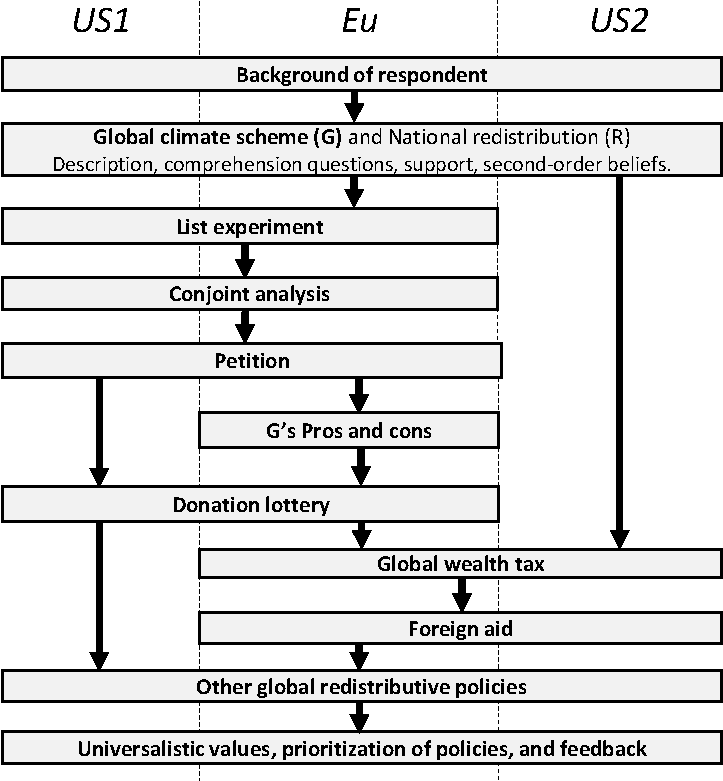
\includegraphics[width=.58\textwidth]{../questionnaire/survey_flow-simple.pdf}} 
\end{figure}

% \begin{table}[h!]
% \renewcommand{\arraystretch}{1.5}
% \caption[Surveys summary]{Summary of the surveys used in the analysis.}
% \label{tab:survey_summary}
% \centering
% \footnotesize
% \begin{tabular}{ |p{2.5cm}|p{3.5cm}|p{2.5cm}|p{2.5cm}|p{3.5cm}|  }
% \cline{2-5}
% \multicolumn{1}{c|}{} & \textbf{Global survey} & \multicolumn{3}{|c|}{\textbf{Complementary surveys}} \\
% \hline
% \textbf{\textit{Name}} & \textit{Global} & \textit{US1} & \textit{US2} & \textit{Eu} \\
% \hline
% \textbf{Region} & 20 high and middle-income countries & U.S. & U.S. & France, Germany, Spain, UK \\
% \hline
% \textbf{Sample size} & 40,680 & 3,000 & 2,000 & 3,000 \\
% \hline
% \textbf{Main purpose} & Stated support for global policies & \multicolumn{3}{|p{8.5cm}|}{Focus on GCS (sincerity, rationales, etc.) + Support for global redistribution + Universalistic values} \\
% % Median duration (in min) & 28 & 20 & 14 & 11 \\ 
% % Date of administration & 03/21--03/22 & 02--03/23 & 01--03/23 & 03--04/23 \\ 
% \hline
% \end{tabular}
% \end{table}

% \renewcommand{\thetable}{S\arabic{table}}
% \begin{table}[h]
%   \caption[Surveys summary]{[For Supplementary Material] Summary of the surveys used in the analysis.}
%   % \caption[Surveys summary]{Characteristics of the different surveys.} 
%   \label{tab:survey_summary}
%   \centering
% \begin{tabular}
%   {@{\extracolsep{5pt}}lcccc} 
%   \\[-1.8ex]\hline 
%   \hline \\[-1.8ex] 
%    & \textit{Global survey} & \multicolumn{3}{c}{\textit{Main surveys}} \\
%   \\[-1.8ex] Survey & \textit{Global} & \textit{Eu} & \textit{US1} & \textit{US2} \\ 
%   \hline \\[-1.8ex]   
%   Country coverage & 20 countries & FR, DE, ES, UK & U.S. & U.S. \\ 
%   Sample size & 40,680 & 3,000 & 3,000 & 2,000 \\ 
%   Main purpose & \makecell{Stated support \\for global policies} & \multicolumn{3}{c}{\makecell{Focus on GCS (sincerity, rationales, etc.) \\+ Support for global redistribution \\+ Universalistic values}} \\
%   % Median duration (in min) & 28 & 20 & 14 & 11 \\ 
%   % Date of administration & 03/21--03/22 & 02--03/23 & 01--03/23 & 03--04/23 \\ 
%   \hline 
%   \hline \\[-1.8ex] 
% \end{tabular}
% \end{table}
% \setcounter{table}{0}
% \renewcommand{\thetable}{\arabic{table}}

\paragraph{Global Survey}

The \textit{Global} survey, conducted in 2021 by Dechezleprêtre et al.,\cite{dechezlepretre_fighting_nodate} involved 40,680 respondents from 20 countries, representing approximately 72\% of global CO$_\text{2}$ emissions. 
This survey serves as the basis for measuring stated support for various global policies worldwide. 
Detailed information about the data collection process, sample representativeness, and analysis of questions on national policies can be found in the companion paper.\cite{dechezlepretre_fighting_nodate}

\paragraph{Main Surveys}\label{par:surveys}

To delve deeper into the sincerity and rationales behind support for the GCS and attitudes towards global policies, global redistribution, and universalistic values, we conducted the Main surveys in 2023. These surveys are based on a sample of 8,000 respondents from France, Germany, Spain, the UK, and the U.S. The European survey (\textit{Eu}) comprises 3,000 respondents, while the U.S. sample was collected in two separate waves: \textit{US1} with 3,000 respondents and \textit{US2} with 2,000 respondents. The survey questions in both the European and U.S. surveys are identical (see Figure \ref{fig:flow_simple}), except for an additional question in \textit{US2} that uses results from \textit{US1} to assess the bandwagon effect.

The Main surveys ensured representativeness along key dimensions: gender, income, age, highest diploma, and degree of urbanization. The \textit{Eu} survey is also representative of its four countries in terms of population size, while the \textit{US1} and \textit{US2} surveys are representative in terms of region and ethnicity. 
Tables \ref{tab:representativeness_waves}-\ref{tab:representativeness_EU} detail how our samples match population frequencies. 
% Tables \ref{tab:representativeness_waves}-\ref{tab:representativeness_EU} confirm that our samples closely match population frequencies. 
More detail on data collection is given in Section \nameref{sec:methods}. The questionnaires used in the surveys are provided in Appendices \ref{app:questionnaire_oecd} and \ref{app:questionnaire}.
% Details regarding the representativeness of the samples are provided in Tables \ref{tab:representativeness_waves}-\ref{tab:representativeness_EU}.



% \subsection{Stated support for global policies}\label{subsec:stated_support}

% The results from both the \textit{Global} and \textit{Complementary} surveys demonstrate robust support for global policies across all surveyed countries, with a clear preference for addressing climate action on a global scale over regional, national, or local approaches.

\subsection{Global support}\label{subsubsec:global_support}

The Global survey shows strong support for climate policies enacted at the global level (Figure \ref{fig:oecd}). %, reproduced from \citealp{dechezlepretre_fighting_nodate}). 
When asked ``At which level(s) do you think public policies to tackle climate change need to be put in place?'', 70\% (in the U.S.) to 94\% (in Japan) choose the global level. The next most popular choice is the federal or continental level, favored by 52\% of Americans and less than half of European respondents. Local policies receive the least support. This preference for climate policies implemented at the global scale is in line with the literature\cite{beiser-mcgrath_could_2019} and consistent with individuals' concerns for the fairness and effectiveness of such policies, which have been identified as two of the three key determinants of support, besides self-interest.\citep{klenert_making_2018,douenne_yellow_2022,dechezlepretre_fighting_nodate} It could also stem from conditional cooperation, although previous studies suggest that the support for climate policies does not depend on climate action abroad.\citep{aklin_prisoners_2020,tingley_conditional_2014}


\begin{figure}[h!]
  % MAJOR figure
  \caption[Relative support for global climate policies]{Support for global climate policies.} 
  \makebox[\textwidth][c]{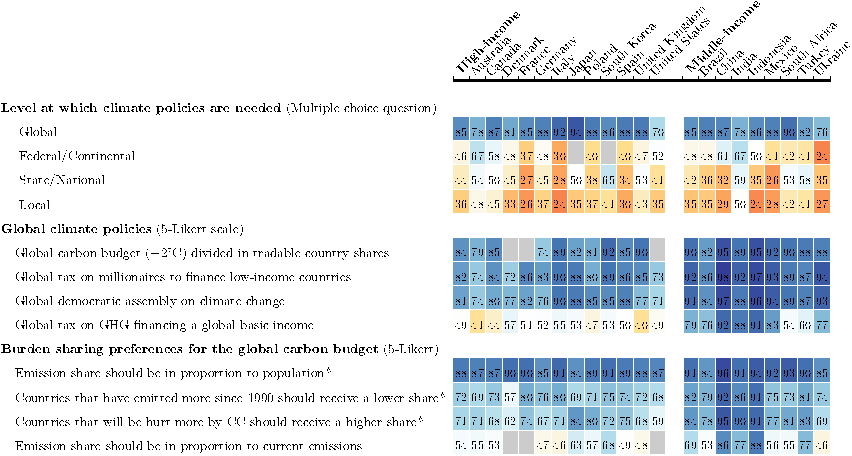
\includegraphics[width=1.2\textwidth]
  {../figures/OECD/Heatplot_global_tax_attitudes_share.pdf}}\label{fig:oecd} % with dependence on others (absent from OECD): Heatplot_burden_share_all_share_countries
  {\footnotesize \\ $\quad$ \\ Note 1: The numbers represent \textit{relative} support, i.e. the share of \textit{Somewhat} or \textit{Strongly support} among non-\textit{indifferent} answers (in percent, $n$ = 40,680). The color blue denotes a relative majority. See Figure \ref{fig:oecd_absolute} for the absolute support. (Questions \ref{q:scale}-\ref{q:millionaire_tax}% Reproduced from \citealp{dechezlepretre_fighting_nodate}, Figure A21.
). \\ Note 2: *In Denmark, France and the U.S., the questions with an asterisk were asked differently, cf. Question \ref{q:burden_sharing_asterisk}. } 
\end{figure}

Among the four global climate policies examined in the \textit{Global} survey, three policies garner high support across all countries (Figure \ref{fig:oecd}). These policies include a global democratic assembly on climate change, a global tax on millionaires to finance low-income countries contingent on their climate action, and a global carbon budget of +2\textdegree{}C divided among countries based on tradable shares (or ``global quota''), with the allocation of country shares unspecified (see wording in Appendix \ref{app:questionnaire_oecd}). 
%\footnote{The policies were all described with further details to make sure people understood them. Specifically, the policies were presented as follows: an international emissions trading system where ``countries that emit more than their national share would pay a fee to countries that emit less than their share''; ``a tax on all millionaires in dollars around the world to finance low-income countries that comply with international standards regarding climate action [which] would finance infrastructure and public services such as access to drinking water, healthcare, and education''; ``a global democratic assembly whose role would be to draft international treaties against climate change [where] each adult across the world would have one vote to elect members of the assembly''.} 
The three policies garner a majority of absolute support (i.e., ``somewhat'' or ``strong'' support) in all countries (except in the U.S. for the global assembly, 48\% absolute support). In high-income countries, the global quota policy obtains 64\% absolute support and 84\% relative support (i.e., excluding ``indifferent'' answers). %Support for this policy is even higher in middle-income countries, however their samples are only representative of the online population (young, graduated and urban people are over-represented).%due to the over-representation of young, educated, and urban populations in the online sample.
% done Several global policies obtain an absolute majority (i.e. \textit{somewhat} or \textit{strong}) %more than 70\% relative % support in all countries
% TODO? remove ", however their samples are only representative of the online population (young, graduated and urban people are over-represented)"

Following the support for the global quota, respondents are asked about their preferences for dividing the carbon budget among countries, as depicted in the third block of Figure \ref{fig:oecd}. Consistent with the existing literature (see Appendix \ref{subsubsec:literature_attitudes_burden_sharing}), an equal per capita allocation of emission rights emerges as the preferred burden-sharing principle, garnering absolute majority support in all countries and never below 84\% relative support. Taking into account historical responsibilities or vulnerability to climate damages is also popular, albeit with less consensus, while grandfathering (i.e., allocation of emission shares in proportion to current emissions) receives the least support in all countries.

A global carbon tax that funds a global basic income should produce the same distributional outcomes as a global tradable quota with equal per capita emission rights (provided that each country returns the revenues from emissions trading equally to its citizens and to the extent that the carbon price is the same). %\footnote{Similarly,  a global quota with grandfathering is equivalent to a global carbon tax where each country keeps the revenues it collects.} 
The support for the global carbon tax is also tested and its redistributive effects --  the average increase in expenditures along with the amount of the basic income -- are specified to the respondents explicitly  (see box below and Appendix \ref{app:questionnaire}, p. \pageref{subsec:questionnaire_GCS}). %: the \$30 per month basic income would lift the 700 million people who earn less than \$2/day out of extreme poverty, and fossil price increases would cost the typical person in their country a certain amount (that is provided).  % The average British person would lose a bit from this policy as they would face £42 per month in price increases, which is higher that the £22 they would receive.
The support for the carbon tax is lower than for the quota, particularly in high-income countries, and there is no relative majority for the tax in Anglo-Saxon countries (consistently with the levels of support found in the only previous study that tested a global carbon tax\cite{carattini_how_2019}). %\footnote{The levels of support are consistent with the findings of \citet{carattini_how_2019}, the only previous study that tested a global carbon tax.} 
Two possible reasons for this lower support are that distributive effects are made salient in the case of the tax, and that people may prefer a quota, perhaps because they find it more effective than a tax to reduce emissions. The combination of both reasons is consistent with the level of support for the global quota once we make the distributive effects salient, as we do in the Main surveys.

% One possible reason for this discrepancy is the explicit emphasis on the redistributive effects associated with the tax in the survey. The survey informs respondents that the \$30 per month basic income would lift 700 million people earning less than \$2/day out of extreme poverty, while fossil price increases would impose costs (specified in the survey) on the typical person in their country. Although other factors such as perceptions of effectiveness may also influence support for a quota versus a tax, this interpretation aligns with the level of support for the global quota when distributive effects are made salient, as we do in the complementary surveys. 

% The remainder of the paper analyzes the results from the complementary surveys in the U.S. and in Europe. This Section covers the stated support for different global redistributive policies. %the Global Climate Scheme, a global wealth tax, other global policies, and foreign aid.

%\subsubsection{Complementary surveys}

% \subsection{The Global Climate Scheme}\label{subsec:gcs}%\label{subsubsec:support_gcs}
%\paragraph{Global Climate Scheme}

\subsection{Stated support for the Global Climate Scheme}\label{subsec:gcs_stated_support}

The Main surveys (\textit{US1}, \textit{US2}, \textit{Eu}) include a comprehensive exploration of citizens' attitudes towards the GCS. We present to respondents a detailed description of the GCS and explain its distributive effects, including specific amounts at stake (as specified in the box below). Furthermore, we assess respondents' understanding of the GCS with incentivized questions to test their comprehension of the expected financial outcome for typical individuals in high-income countries (loss) and the poorest individuals globally (gain), followed by the provision of correct answers (Figures \ref{fig:understood_each}-\ref{fig:understood_score}). % TODO? That is, respondents are made aware and we find they understand that the policy will make people in their country poorer. 
% TODO? . 63\% understand the policy will make people in their country poorer, before even we indicate this as the right answer.
The same approach is applied to a National Redistribution scheme (NR) targeting top incomes % the top 5\% (in the U.S.) or top 1\% (in Europe) 
with the aim of financing cash transfers to all adults, %\footnote{The wider base in the U.S. was chosen because emissions are larger in the U.S. than in Europe, and it would hardly be feasible to offset the median American's loss by taxing only the top 1\%.} 
calibrated to offset the monetary loss of the GCS for the median emitter in their country. We evaluate respondents' understanding that the richest would lose and the typical fellow citizens would gain from that policy. % done We proceed the same way for a National Redistribution Scheme (NR) that would tax the top 5\% (in the U.S.) or the top 1\% (in Europe) to finance cash transfers to all adults (calibrated to offset the monetary loss of the GCS for the median emitter), expecting people to find out at the comprehension question that the richest would lose and the typical people in their country would win.
Subsequently, we summarize both schemes to enhance respondents' recall. Additionally, we present a final incentivized comprehension question and provide the expected answer that the combined GCS and NR would result in no net gain or loss for a typical fellow citizen. Finally, respondents are directly asked to express their support for the GCS and NR using a simple \textit{Yes}/\textit{No} question.

\begin{tcolorbox}\label{box:GCS}
  \paragraph{The Global Climate Scheme} The GCS consists of global emissions trading with emission rights being auctioned each year to polluting firms, and of a global basic income, funded by the auction revenues. Using the price and emissions trajectories from the report by Stern \& Stiglitz,\cite{stern_report_2017} and in particular a carbon price of \$90/tCO$_\text{2}$ in 2030, we estimate that the basic income would amount to \$30 per month for every human adult %over the age of 15 
  (see details in Appendix \ref{app:gain_gcs}). %, enough to lift out of extreme poverty the 700 million people who live with less than PPP \$2 per day. Conversely, assuming a carbon price of \$90/tCO$_\text{2}$ in 2030, high emitters like a typical American (with median U.S. CO$_\text{2}$ emissions) would lose in net \$85 per month, as they would face \$115 per month in price increases (see details in Appendix \ref{app:gain_gcs}). 
  We describe the GCS to the respondents as a ``climate club'' and we specify its redistributive effects: The 700 million people with less than \$2/day [in Purchasing Power Parity] would be lifted out of extreme poverty, and fossil fuel price increases would cost the typical person in their country a specified amount (see Appendix \ref{subsec:questionnaire_GCS} for details). The monthly median net cost is \$85 in the U.S., \euro{}10 in France, \euro{}25 in Germany, \euro{}5 in Spain, £20 in the UK.
\end{tcolorbox}

The stated support for the GCS is 54\% in the U.S. and 76\% in Europe, while the support for NR is very similar: 56\% and 73\% respectively (see Figure \ref{fig:support_binary}). 
% The 95\% confidence intervals are $[52.4\%, 55.9\%]$ in the U.S. and $[74.2\%, 77.2\%]$ in Europe. The average support is computed with survey weights, employing weights based on quota variables, which exclude vote. Another method to reweigh the raw results involves running a regression of the support for the GCS on sociodemographic characteristics (including vote) and multiplying each coefficient by the population frequencies. This alternative approach yields similar figures: 76\% in Europe and 52\% or 53\% in the U.S. (depending on whether individuals who did not disclose their vote are classified as non-voters or excluded). Notably, the average support excluding non-voters is 54\% in the U.S.
Appendix \ref{app:determinants} examines the sociodemographic determinants of support for the GCS as well as the beliefs correlated with the support for a global tax on GHG financing a global basic income. The strongest correlates are political leaning, trust in the government and perceptions that the policy is effective at reducing emissions or in one's self-interest. %presents the sociodemographic determinants of GCS support, showing, for instance, stronger support among young people.
% Supplementary Section F examines the sociodemographic determinants of support for the GCS as well as the beliefs correlated with the support for a global tax on GHG financing a global basic income. The strongest correlates are political leaning, trust in the government and perceptions that the policy is effective at reducing emissions or in one's self-interest.

% \setcounter{figure}{0}
% \renewcommand{\thefigure}{S\arabic{figure}}
% \begin{figure}[h!]
%     \caption[Support for the Global Climate Scheme]{[For Supplementary Material, except first row to be included in Figure \ref{fig:support}] Support for the GCS, NR and the combination of GCS, NR and C (\textit{Yes}/\textit{No} questions). \\(p. \pageref{subsec:questionnaire_GCS}, Questions \ref{q:gcs_support}, \ref{q:nr_support}, \ref{q:global_tax}, \ref{q:national_tax}, and \ref{q:crg_support}).%; $n_\text{US} = n_\text{Eu} = 3,000,\, n_\text{FR} = 729,\, n_\text{DE} = 929,\, n_\text{ES} = 543,\, n_\text{UK} = 749$)
%     }\label{fig:support_binary}
%     \makebox[\textwidth][c]{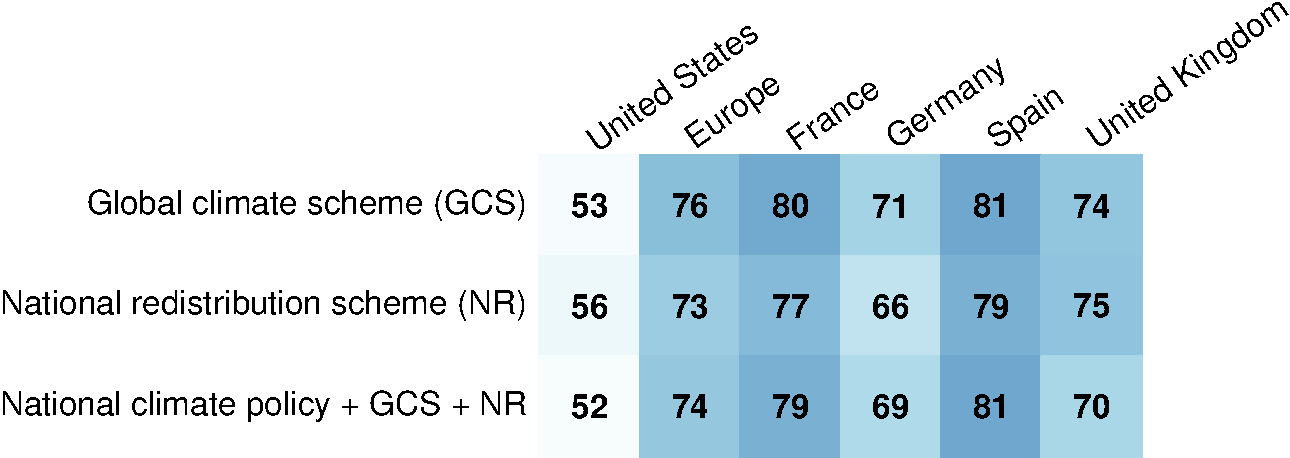
\includegraphics[width=.9\textwidth]{../figures/country_comparison/support_binary_positive.pdf}} 
% \end{figure}


\subsection{Robustness and sincerity of support for the GCS}\label{subsec:robustness_sincerity}


We use several methods to assess the sincerity of the support for the GCS: a list experiment, a real-stake petition, conjoint analyses, and the prioritization of policies. All methods suggest that the support is either completely sincere, or the share of insincere answers is limited. 

\subsubsection{List experiment}\label{subsubsec:list_exp} % NCCcomment

% A list experiment is employed to gauge tacit support for a specific policy of interest by asking respondents how many policies within a given list they support. By varying the list among respondents, the difference in number of policies supported can be used to estimate tacit support, revealing potential social desirability biases \citep{hainmueller_causal_2014}.
By asking \textit{how many} policies within a list respondents support and varying the list among respondents, a list experiment allows identifying the tacit support for a policy of interest. 
% The tacit support is estimated as the difference in the average number of policies supported between two groups, whose list differ only by the inclusion of that policy.\citep{hainmueller_causal_2014} % respondents who face a list containing the policy, and respondents who face the same list without it. 
For example, say a first subsample faces the list of policies A, B, and C, while a second subsamples faces the list A, B, C, and GCS. We do not need to know which policies each respondent support to estimate the average (tacit) support for the GCS, we simply need to compute the difference in the average number of supported policies between the two random subsamples.\citep{imai_multivariate_2011} 
% List experiments have been used to reveal social desirability bias, silencing either racism in the Southern U.S.\citep{kuklinski_racial_1997} or opposition to the invasion of Ukraine in Russia.\citep{chapkovski_solid_2022} % TODO? remove?
In our case, as shown in Table \ref{tab:list_exp}, the tacit support for the GCS measured through the list experiment is not significantly lower than the direct stated support. %\footnote{We utilize the difference-in-means estimator, and confidence intervals are computed using Monte Carlo simulation with the R package \textit{list}.\citep{imai_multivariate_2011}} 
Hence, we do not find a social desirability bias in our study.

% The tacit support for the GCS measured through the list experiment is as high as  the direct question in Eu but significantly lower by 5 p.p. in the U.S. This may be the sign of a social norm pushing some Americans to state that they support the GCS although they secretly do not. Still, if there is a social norm in favor of the GCS, there is a similar norm in favor of the National Redistribution Scheme, as the gap between the tacit and direct support for it is comparable (at 6 p.p.). %However, two observations qualify this interpretation. First, the gap between the tacit and direct support for the National Redistribution Scheme is comparable (at 7 p.p.) though we did not expect such a social norm in the case of the national redistribution, as the 95\% who would benefit from it should not feel ashamed to oppose a policy that would benefit them. Second, while we tested the questionnaire on random people in cafés, we noticed that some were confused by the question of the list experiment (asking how many policies from the list they supported), upset with the conservative societal policy (``Marriage only for opposite-sex couples in the U.S.'', ``Death penalty for major crimes'' in Europe), to the point that they did not answer attentively.

% \begin{table}[h]
%   % MAJOR figure % TODO! same table for NR in appendix
%   % TODO table by country
%   \caption[List experiment: tacit support for the GCS]{Number of supported policies in the list experiment depending on the presence of the Global Climate Scheme (GCS) in the list. %in function of the composition of the list. GCS stands for the Global Climate Scheme and NR for the National Redistribution Scheme.} % Beware, this question is quite unusual. \\ Among the policies below, how many do you support?  \\ Coal exit, Marriage only for opposite-sex couples 
%    The tacit support for the GCS is estimated by regressing the number of supported policies on the presence of the GCS in the list of policies. The social desirability is estimated as the difference between the tacit and stated support, and it is not significantly different from zero even at a 20\% threshold (see \nameref{sec:methods}).
%   }\label{tab:list_exp}
%   \makebox[\textwidth][c]{
\begin{tabular}{@{\extracolsep{5pt}}lccc} 
\\[-1.8ex]\hline 
\hline \\[-1.8ex] 
 & \multicolumn{3}{c}{Number of supported policies} \\ 
\cline{2-4} 
\\[-1.8ex] & All & US & Europe \\ 
\hline \\[-1.8ex] 
 List contains: GCS & 0.624$^{***}$ & 0.524$^{***}$ & 0.724$^{***}$ \\ 
  & (0.028) & (0.041) & (0.036) \\ 
\hline  \\[-1.8ex] \textit{Support for GCS} & 0.65  &  0.542  &  0.757 \\
\textit{Social desirability bias} & \textit{$ -0.026 $} & \textit{$ -0.018 $} & \textit{$ -0.033 $}\\
\textit{80\% C.I. for the bias} & \textit{ $[ -0.06 ; 0.01 ]$ } & \textit{ $[ -0.07 ; 0.01 ]$} & \textit{ $[ -0.08 ; 0.01 ]$}\\
 \hline \\[-1.8ex] 
Constant & 1.317 & 1.147 & 1.486 \\ 
Observations & 6,000 & 3,000 & 3,000 \\ 
R$^{2}$ & 0.089 & 0.065 & 0.125 \\ 
\hline 
\hline \\[-1.8ex] 
\textit{Note:}  & \multicolumn{3}{r}{$^{*}$p$<$0.1; $^{**}$p$<$0.05; $^{***}$p$<$0.01} \\ 
\end{tabular} 
%   }  
%   % {\footnotesize \textit{Note:} $^{*}p<0.1$; $^{**} p<0.05$; $^{***} p<0.01$.}
% \end{table}

% Donation addresses experimenter demand
\subsubsection{Petition}\label{subsubsec:petition} % Addresses hypothetical bias  % NCCcomment

% H1: Petition: Small effect against GCS: -4pp
We ask respondents whether they are willing to sign a petition in support of either the GCS or NR policy. We inform them that the petition results will be sent to the head of state's office, highlighting the proportion of fellow citizens endorsing the respective scheme. Even when framed as a petition that might have real stakes, both policies continue to receive majority support. In the U.S., we find no significant difference between the support in the %real-stake 
petitions and the simple questions (GCS: $p=.30$; NR: $p=.76$). %\footnote{Paired weighted \textit{t}-tests are conducted to test the equality in support for a policy among respondents who were questioned about the policy in the petition.} 
In Europe, the petition leads to a comparable lower support for both the GCS (7 p.p., $p=10^{-5}$) and NR (4 p.p., $p = .008$). While some European respondents are unwilling to sign a petition for policies they are expected to support, this phenomenon is not specific to the GCS, and the overall willingness to sign a %real-stake 
petition remains strong, with 69\% expressing support for the GCS and 67\% for NR.

\subsubsection{Conjoint analyses}\label{subsubsec:conjoint} % Addresses acquiescence bias  % NCCcomment
% H1, H2: Conjoint analysis: G|C+R 56%, G|R 59%, G 48% ~ C (|R), G+C|R 56%, C|R 64%, Left+G - Left = -3pp, A+G vs. B 59%
% => G is supported for itself, rather independently from R or C, with similar support to both, and it doesn't significantly penalize the Left, and would help a Democratic candidate

In order to assess the public support for the GCS in conjunction with other policies, we conduct a series of conjoint analyses. We ask respondents to make five choices between pairs of political platforms.

The first conjoint analysis suggests that the GCS is supported independently of being complemented by the National Redistribution Scheme and a national climate policy (C). % (``Coal exit'' in the U.S., ``Thermal insulation plan'' in Europe, denoted C).
%\footnote{Indeed, 54\% of %($n$ = 3,000) 
% U.S. respondents and 74\% of %($n$ = 3,000) 
% European ones prefer the combination of C, NR and the GCS to the combination of C and NR alone, indicating similar support for the GCS conditional on NR and C than for the GCS alone (Figure \ref{fig:conjoint}).} % (as it does not significantly differ from the direct support of 53\%). 
% For the second analysis, we split the sample into four random branches (see \nameref{sec:methods}). 
% % \footnote{Results from the first branch show that the support for the GCS conditional on NR, at 55\% in the U.S. ($n$ = 757) and 77\% in Europe ($n$ = 746), is not significantly different from the support for the GCS alone. This suggests that rejection of the GCS is not driven by the cost of the policy on oneself. The second branch shows that the support for C conditional on NR is somewhat higher, at 62\% in the U.S. ($n$ = 751) and 84\% in Europe ($n$ = 747). However, the third one shows no significant preference for C compared to GCS (both conditional on NR), neither in Europe, where GCS is preferred by 52\% ($n$ = 741) nor in the U.S., where C is preferred by 53\% ($n$ = 721). The fourth branch shows that 55\% in the U.S. ($n$ = 771) and 77\% in Europe ($n$ = 766) prefer the combination of C, NR and the GCS to NR alone.} 
% The outcome is that there is
The second analysis indicates majority support for the GCS and for C, which are seen as neither complement nor substitute (see \nameref{sec:methods}). A minor share of respondents like a national climate policy and dislike a global one, but as many people prefer a global rather than a national policy; and there is no evidence that implementing NR would increase the support for the GCS.


In the third analysis, we present two random branches of the sample with hypothetical progressive and conservative platforms that differ only by the presence (or not) of the GCS in the progressive platform. Table \ref{tab:conjoint_c} shows that a progressive candidate would not significantly lose voting share by endorsing the GCS in any country, and may even gain 11 p.p. ($p = .005$) in voting intention in France. %The effect is also positive at 3 p.p. ($p = .13$) in the U.S., although not significant at the 5\% threshold. % France holds multiple hypotheses testing

% Though the level of support for the GCS is significantly lower in swing States (at 51\%) that are key to win U.S. elections, the electoral effect of endorsing the GCS remains non-significantly different from zero (at +1.2 p.p.) in these States.
% \footnote{We define swing states as the 8 states with less than 5 p.p. margin of victory in the 2020 election (MI, NV, PA, WI, AZ, GA, NC, FL). The results are robust to using the 3 p.p. threshold (that excludes FL) instead.}

%The third analysis suggests that a progressive candidate would not significantly lose voting share if he or she were to endorse the GCS, and that he or she may even gain 11 p.p. vote intention in France (see Table \ref{tab:conjoint_c}). To estimate this, we present to two random branches of the sample hypothetical progressive and conservative platforms that differ only by the presence (or not) of the GCS in the progressive platform. 

% \begin{table}[h]
%   % MAJOR figure
%   \caption[Influence of the GCS on electoral prospects]{Preference for a progressive platform depending on whether it includes the GCS or not. (Question \ref{q:conjoint_c}) 
%   %Imagine if the [Democratic and Republican presidential candidates in 2024] campaigned with the following policies in their platforms. [Credible Progressive and Conservative platforms] \\ % TODO See More
% % Which of these candidates would you vote for? \textit{A; B; None of them} \\
% % ~[FR: second round of presidential; DE, ES, UK: two favorite candidates in one's constituency]
% } % Beware, this question is quite unusual. \\ Among the policies below, how many do you support?  \\ Coal exit, Marriage only for opposite-sex couples 
%   \makebox[\textwidth][c]{
\begin{tabular}{@{\extracolsep{5pt}}lcccccc} 
\\[-1.8ex]\hline 
\hline \\[-1.8ex] 
 & \multicolumn{6}{c}{Prefers the Progressive platform} \\ 
\cline{2-7} 
\\[-1.8ex] & All & United States & France & Germany & UK & Spain \\ 
\hline \\[-1.8ex] 
 GCS in Progressive platform & 0.028$^{*}$ & 0.029 & 0.112$^{***}$ & 0.015 & 0.008 & $-$0.015 \\ 
  & (0.014) & (0.022) & (0.041) & (0.033) & (0.040) & (0.038) \\ 
 \hline \\[-1.8ex] 
Constant & 0.623 & 0.604 & 0.55 & 0.7 & 0.551 & 0.775 \\ 
Observations & 5,202 & 2,619 & 605 & 813 & 661 & 504 \\ 
R$^{2}$ & 0.001 & 0.001 & 0.013 & 0.0003 & 0.0001 & 0.0003 \\ 
\hline 
\hline \\[-1.8ex] 
\end{tabular} 
}\label{tab:conjoint_c}
%   {\footnotesize \textit{Note:} Simple OLS model. The 14\% of \textit{None of them} answers have been excluded from the regression samples. GCS has no significant influence on them. $^{*}p<0.1$; $^{**} p<0.05$; $^{***} p<0.01$. 
%   }
% \end{table}
% \begin{stretchpars}

Our last two analyses  make respondents choose between two random platforms. In Europe, respondents are prompted to imagine that a left or center-left coalition will win the next election and asked what platform they would prefer that coalition to have campaigned on. In the U.S., the question is framed as a hypothetical duel in a Democratic primary, and asked only to non-Republicans ($n$ = 2,218), i.e. the respondents who declare as political affiliation \textit{Democrat}, \textit{Independent}, \textit{Non-Affiliated} or \textit{Other}. In the fourth analysis, a policy (or an absence of policy) is randomly drawn for each platform in each of five categories: \textit{economic issues}, \textit{societal issues}, \textit{climate policy}, \textit{tax system}, \textit{foreign policy} (Figure \ref{fig:ca_r}). 

% Except for the category \textit{foreign policy}, which features the GCS 42\% of the time, the policies are prominent progressive policies and they are drawn uniformly. % except for tax1: .35 vs. tax2: .4 in EU. 
In the UK, Germany, and France, a platform is about 9 to 13 p.p. more likely to be preferred if it includes the GCS rather than no foreign policy. %\footnote{This is the Average Marginal Component Effect.\cite{hainmueller_causal_2014}} 
This effect is between 1 and 4 p.p. and no longer significant in the U.S. (among non-Republicans) and in Spain. Moreover, a platform that includes a global tax on millionaires rather than no foreign policy is 5 to 13 p.p. more likely to be preferred in all countries (the effect is significant and at least 9 p.p. in all countries but Spain). 
% Moreover, a platform that includes a global tax on millionaires rather that no foreign policy is 9 to 13 percentage points (p.p.) more likely to be preferred in all countries but Spain (not significant, at +5 p.p.). 
Similarly, a global democratic assembly on climate change has a significant effect of 8 to 12 p.p. in the U.S. (among non-Republicans), Germany, and France. 
%In each country, a platform is more likely to be preferred if it includes the GCS rather than no foreign policy. This effect is significant in France, Germany and the UK, where a platform is about 10 p.p. more likely to be preferred. 
These effects are large, and not far from the effects of the policies most influential on the platforms, which range between 15 and 18 p.p. in most countries (and 27 p.p. in Spain), and all relate to improved public services (in particular healthcare, housing, and education).
% \end{stretchpars}
 
% \begin{figure}[h] 
%   \caption[Preferences for various policies in political platforms]{[For Supplementary Material] Effects of the presence of a policy (rather than none from this domain) in a random platform on the likelihood that it is preferred to another random platform. (See non-translated versions in Figure \ref{fig:ca_r_en}; Question \ref{q:conjoint_r}%; in the U.S., asked only to non-Republicans.
%   )}\label{fig:ca_r}
%   \begin{subfigure}{\textwidth}
%     \subcaption{U.S. (Asked only to non-Republicans)}
%     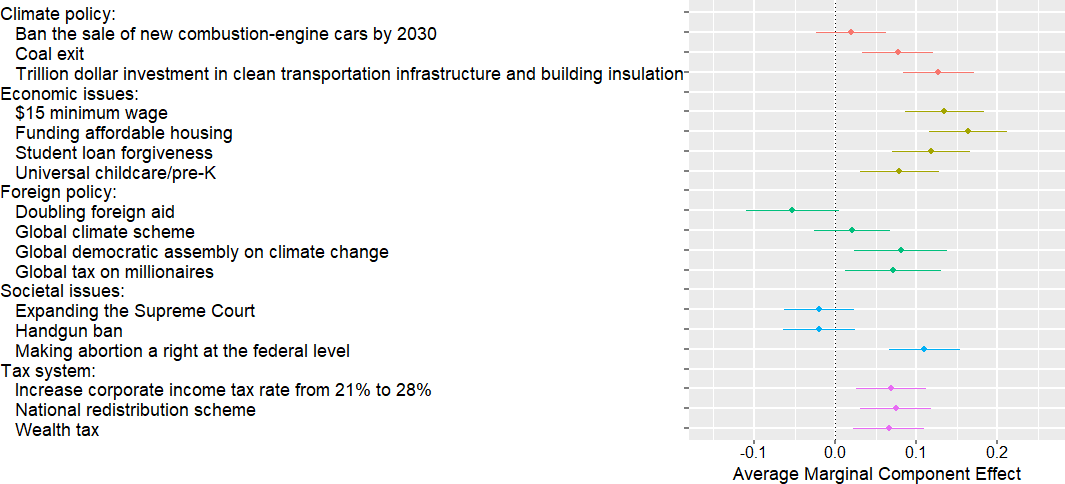
\includegraphics[width=\textwidth]{../figures/US1/ca_r.png}
%   \end{subfigure}
%   \begin{subfigure}{\textwidth}
%     \subcaption{France}
%     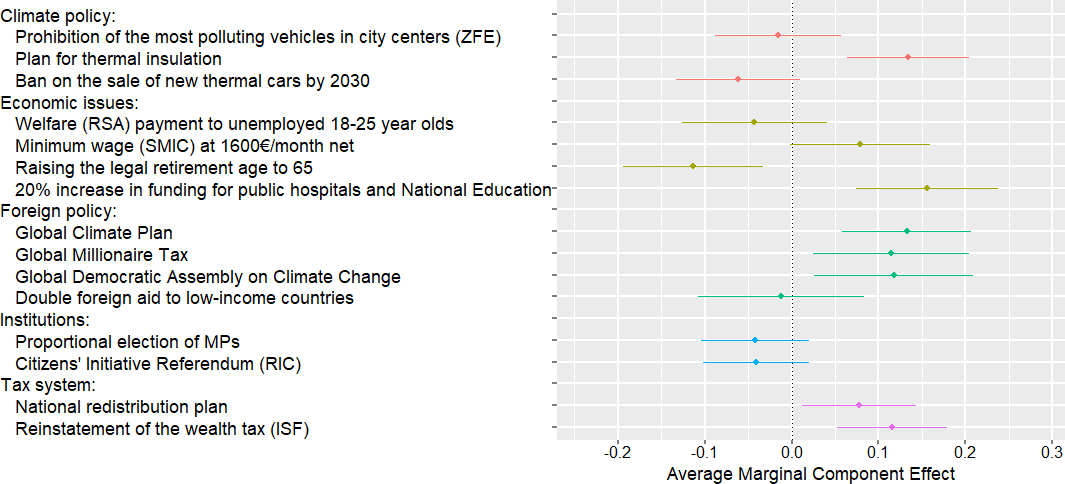
\includegraphics[width=\textwidth]{../figures/FR/ca_r_en.png}
%   \end{subfigure}
% \end{figure}%
% \clearpage
% \begin{figure}[h!]\ContinuedFloat % if bugs try b! instead of h!
%   \begin{subfigure}{\textwidth}
%     \subcaption{Germany}
%     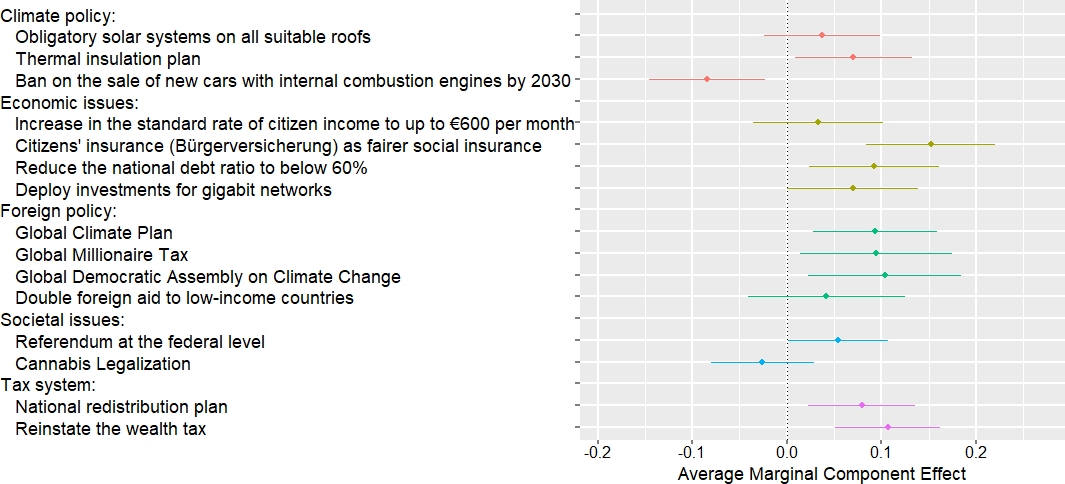
\includegraphics[width=\textwidth]{../figures/DE/ca_r_en.png}
%   \end{subfigure}
%   \begin{subfigure}{\textwidth}
%     \subcaption{Spain}
%     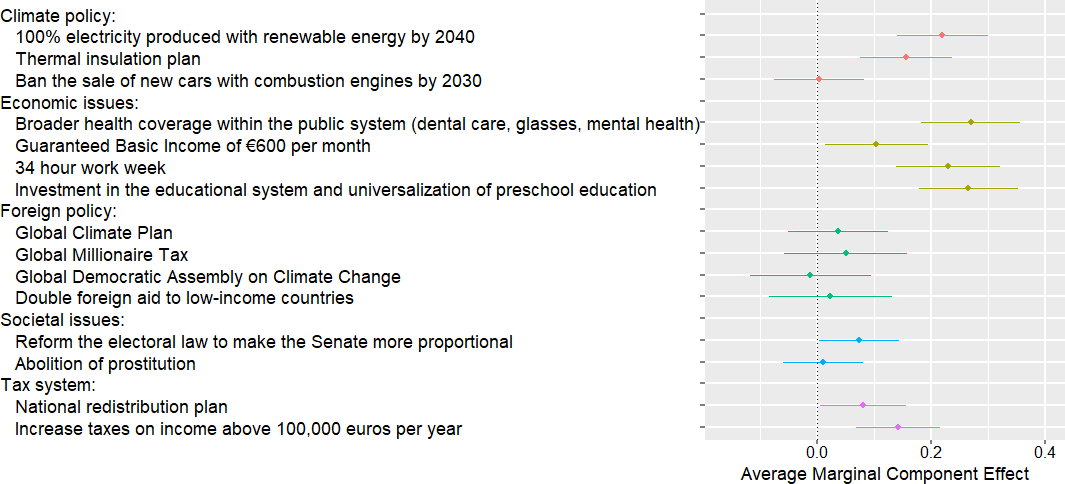
\includegraphics[width=\textwidth]{../figures/ES/ca_r_en.png}
%   \end{subfigure}
%   \begin{subfigure}{\textwidth}
%     \subcaption{UK}
%     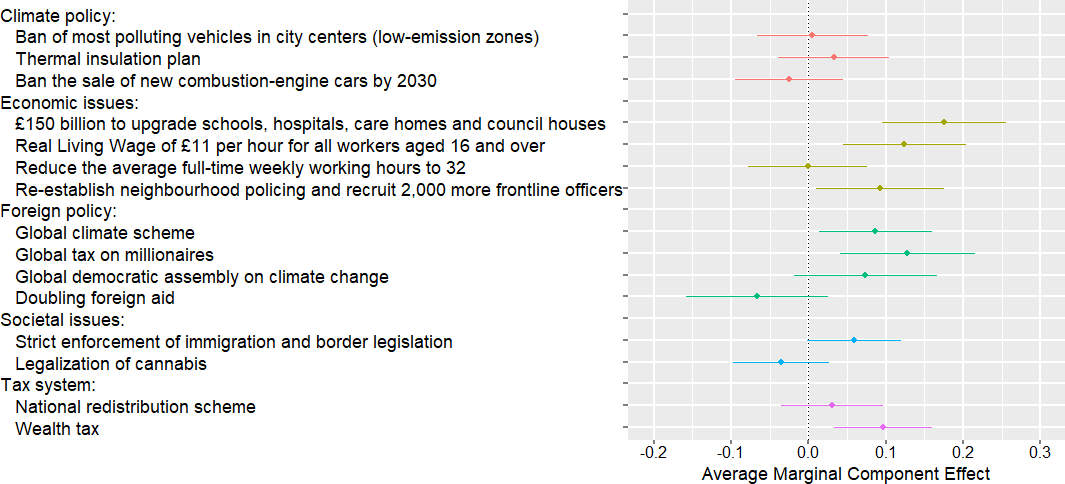
\includegraphics[width=\textwidth]{../figures/UK/ca_r.png}
%   \end{subfigure}
%   %\makebox[\textwidth][c]{} 
% \end{figure}
% \clearpage 
% \noindent 
The fifth analysis draws random platforms similarly, except that candidate A's platform always contains the GCS while B's includes no foreign policy. In this case, A is chosen by 60\% of Europeans %($n$ = 3,000) 
and 58\% of non-Republican Americans (Figure \ref{fig:conjoint_left_ag_b}). %($n$ = 2,218). 
Overall, taking the U.S. as an example, our conjoint analyses indicate that a candidate at the Democratic primary would have more chances to obtain the nomination by endorsing the GCS, and this endorsement would not penalize her or him at the presidential election. 
% This result reminds the finding that 12\% of Germans shift their voting intention from SPD and CDU/CSU to the Greens and the Left when they are told that the latter parties support global democracy.\citep{ghassim_who_2020}


% \begin{figure}[h!]
%     \caption[Influence of the GCS on preferred platform]{[For Supplementary Material] Influence of the GCS on preferred platform:\\ Preference for a random platform A that contains the Global Climate Scheme rather than a platform B that does not (in percent). (Question \ref{q:conjoint_d}; in the U.S., asked only to non-Republicans.)}\label{fig:conjoint_left_ag_b}
%     \makebox[\textwidth][c]{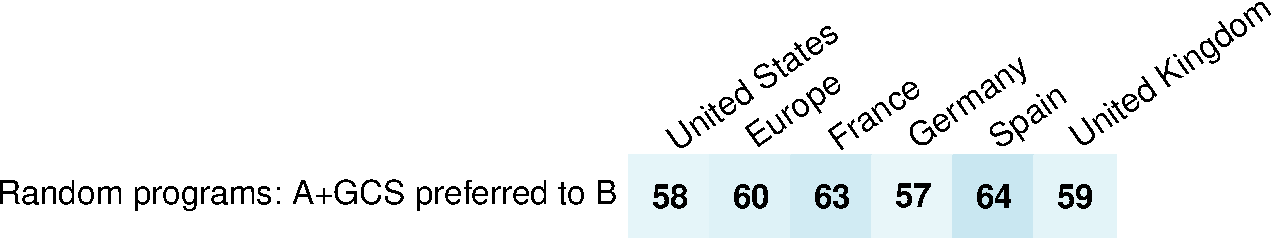
\includegraphics[width=\textwidth]{../figures/country_comparison/conjoint_left_ag_b_binary_positive.pdf}} 
% \end{figure}


% \begin{figure}
%   % Imagine that at the 2024 Democratic party presidential primaries, the two main candidates campaign with the following key policies in their platforms. \\ Which of these candidates do you prefer?

%   \caption{Conjoint analysis. Average Marginal Component Effects (relative to the baseline: an absence of policy of that category) of policies in the choice between two platforms, where policies in each platform are randomly drawn ($n$ = 6,000). In Eu, it is framed as two potential platforms of a left-wing coalition that would win the next elections; in the U.S., it is framed as a hypothetical duel in the 2024 Democratic primary and asked only to non-Republicans.}\label{fig:ca_r} % TODO: add ref to Question
%   \makebox[\textwidth][c]{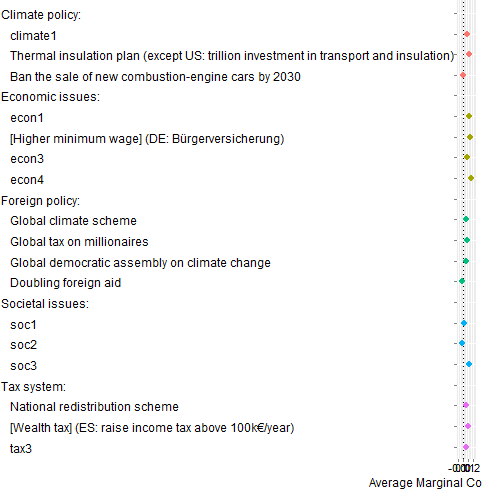
\includegraphics[width=\textwidth]{../figures/all/ca_r.png}}
% \end{figure}

\subsubsection{Prioritization}\label{subsubsec:prioritization} % Addresses acquiescence bias and social desirability bias
% H1: Prioritization: G has mean only slightly lower than average, makes better than ban of cars and coal exit; global tax on millionaires does as well as wealth tax and almost as good as $15 minimum wage

Towards the end of the survey, we ask respondents to allocate 100 points among six randomly selected policies from the previous conjoint analyses, using sliders. The instruction was to distribute the points based on their level of support, with a higher allocation indicating greater support for a policy. %At the end of the survey, we pick six policies at random (and uniformly) among the policies used in the last conjoint analyses, and ask respondents to allocate 100 points among them (using sliders), with the instruction that ``the more you give points to a policy, the more you support it''. 
As a result, the average support across policies is 16.67 points. %(Figure \ref{fig:points}). % TODO! figures for each country
In each country, the GCS ranks in the middle of all policies or above, with an average number of points from 15.4 in the U.S. to 22.9 in Germany.%The GCS ranked in the middle or higher among all policies in each country, receiving an average of 15.4 points in the U.S. and 22.9 points in Germany.

Interestingly, in Germany, the most prioritized policy is the global tax on millionaires, while the GCS is the second most prioritized policy. The global tax on millionaires consistently ranks no lower than fifth position (out of 15 or 17 policies) in every country, garnering an average of 18.3 points in Spain to 22.9 points in Germany.

% This question sheds light on a potential discrepancy between the policy priorities of the public and those enacted by legislators. For instance, while the European Union and California have enacted plans to phase out new combustion-engine cars by 2035, the proposal to ``ban the sale of new combustion-engine cars by 2030'' emerged as one of the three least prioritized policies in each country, with an average allocation of 7.8 points in France to 11.4 points in the UK.

%It is higher than to ``ban the sale of new combustion-engine cars by 2030'' (13.4) and ``coal exit'' (10.0), but lower than the third climate policy: ``trillion dollar investment in clean transportation infrastructure and building insulation'' (20.3). The support for other globally redistributive policies is variable: ``Doubling foreign aid'' is the least supported policy (8.4), while the ``Global tax on millionaires'' is one of the five policies with more than 20 points (20.2), and the ``global democratic assembly on climate change'' is just below the GCS (14.5). The most supported policies are ``Funding affordable housing'' (28.5), ``\$15 minimum wage'' (23.8), and ``Universal childcare/pre-K'' (22.1). % TODO? share that allocated at least 1

% \begin{figure}[h!]
%   \caption{Prioritization of policies. Each respondent faces six policies taken at random from the ones below and allocates 100 points among them to signal the strength of their support for each one ($n$ = 3,000).} % Imagine you have 100 points that you can allocate to different policies. The more you give points to a policy, the more you support it.  \\  How do you allocate the points among the following policies?  
  
%   \makebox[\textwidth][c]{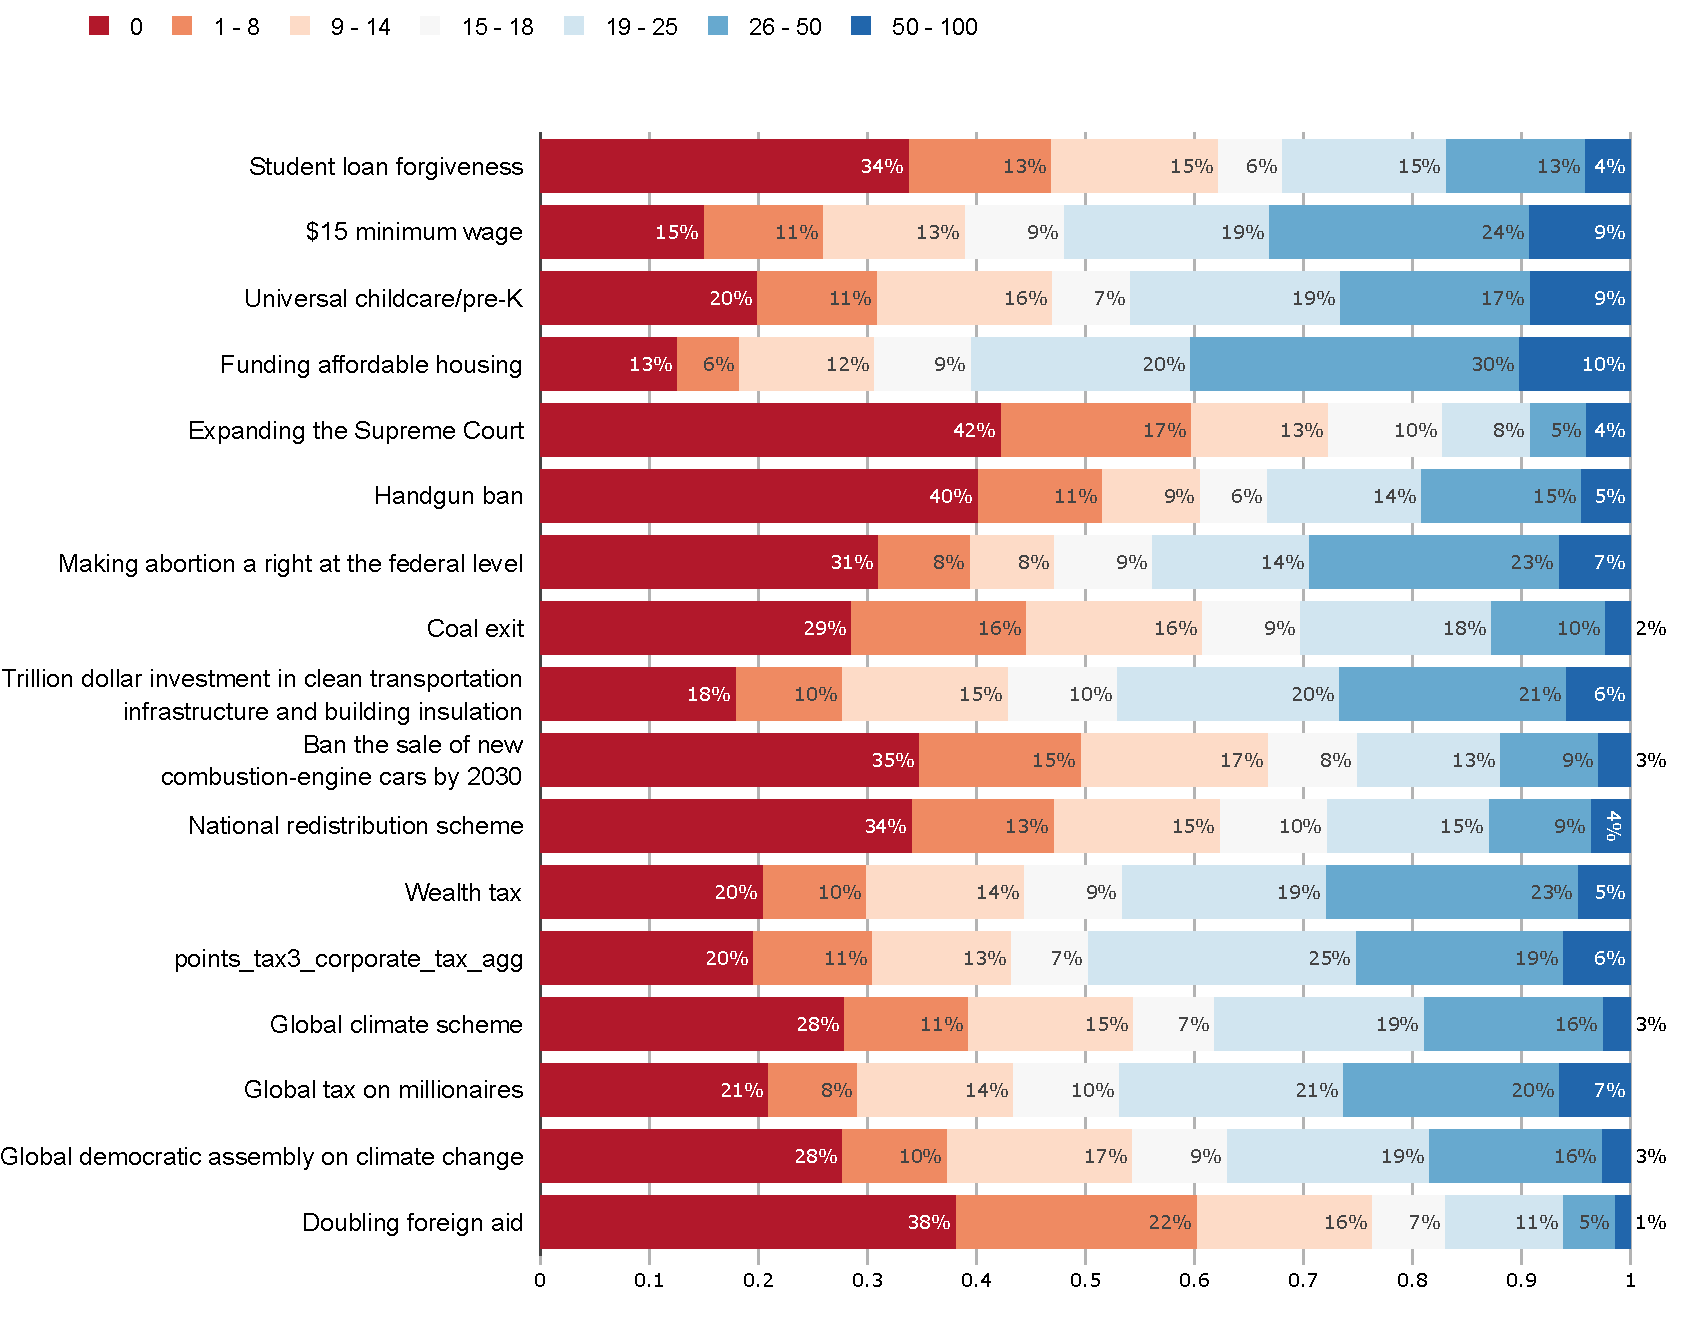
\includegraphics[width=\textwidth]{../figures/US1/points_us.pdf}}\label{fig:points}
% \end{figure}

% TODO? This slightly differs from a conjoint analysis, which only allows inferring individual-level preferences for one platform over another or collective-level preferences for one policy over another. Also, by comparing platforms, conjoint analyses may be subject to interaction effects between policies of a platform (which can be seen as Main, subsitute, or antagonistic) while the prioritization frames the policies as independent.

\subsubsection{Pros and Cons}\label{subsubsec:pros_cons}

We survey respondents to gather their perspectives on the pros and cons of the GCS, randomly utilizing an open-ended or a closed question. In the closed question format, respondents tend to consider every argument as important in determining their support or opposition to the GCS (see Figure \ref{fig:gcs_important}). 
% Notably, the least important aspect was the negative impact on their household, with 60\% in Europe ($n$=1,505) and 75\% in the U.S. ($n$=493) finding it important. The most important elements differ between Europe and the U.S. In Europe, the key factors are the GCS's potential to limit climate change and reduce poverty in low-income countries, both deemed important by 85\% of respondents. In the U.S., having sufficient information about the scheme ranks highest at 89\%, followed by its potential to foster global cooperation at 82\%. However, d
% Due to the limited variation in the ratings for each element, the closed question format is inconclusive (Figure \ref{fig:gcs_important}). % TODO? distinguish between supporters and opponents?
% TODO? cite figure 

The open-ended question provides more insights into what people associate with the GCS when prompted to think about it. % The open-ended question gives interesting insight into ``what comes to [people's] mind'' when ``thinking of the GCS''. 
Analyzing keywords in the responses (automatically translated into English), the most frequently mentioned topics are the international aspect and the environment, each appearing in approximately one-quarter of the answers (see Figure \ref{fig:gcs_field_contains}). This is followed by discussions on the effects of the GCS on poverty and prices, each mentioned by about one-tenth of the respondents. We also manually classified each answer into different categories (see Figure \ref{fig:gcs_field}). This exercise confirms the findings from the automatic search: the environmental benefit of the GCS is the most commonly discussed topic, while obstacles to implementation or agreement on the proposal are relatively infrequently mentioned.%the most frequent topic is the environmental benefit of the GCS, while the obstacles to implement it or to get %people or countries agreement on it are relatively seldom mentioned.
% \footnote{Moreover, around one in four respondents explicitly cites pros or cons. Few individuals explicitly express support or opposition, and misunderstandings are rare. Only 11\% of the responses are empty or express a lack of opinion, though one-quarter are unclassifiable due to the rarity, nonsensical nature, or irrelevance of the conveyed idea.}% TODO n

% In the \textit{US2} survey, we presented these questions to random subsamples \textit{before} inquiring about support for the GCS or NR. The sample was divided into four branches: two branches with questions on pros and cons (either in closed or open form), one branch providing information on the actual level of support for the GCS and NR (estimated in \textit{US1}), and one control group without these questions.\footnote{Consistent with Americans accurately perceiving the levels of support for the GCS or NR, providing information on the actual level had no substantial effect on their support. In the closed question regarding pros and cons, we intentionally included more cons (6) than pros (3) to conservatively estimate the potential campaign effect on the GCS, which refers to the shift in opinion resulting from media coverage of the proposal. Interestingly, the support for the GCS decreased by 11 p.p. after respondents viewed a list of its pros and cons. Surprisingly, the support for National Redistribution also decreased by 7 p.p. following the closed question about the GCS. This suggests that some individuals may lack attention and confuse the two policies, or that contemplating the pros and cons alters the mood of some people, moving them away from their initial positive impression. Notably, the support also decreased by 7 p.p. after respondents were asked to consider the pros and cons in an open-ended question.} Despite some significant effects of pondering the pros and cons (see Table \ref{tab:branch_gcs}), approximately half of the Americans expressed support for the GCS across all treatment branches. If similar effects were observed in Europe, it suggests that the GCS would still enjoy strong majority support among Europeans once it enters the public debate (Table \ref{tab:branch_gcs}).


In the \textit{US2} survey, we divided the sample into four random branches. Two branches were presented the pros and cons questions (either in open or closed format) \textit{before} being asked about their support for the GCS or NR. Another branch received information on the actual level of support for the GCS and NR (estimated in \textit{US1}, see box p. \pageref{subsec:second_order_beliefs}), %Section \ref{subsec:second_order_beliefs}), 
and one control group received none of these treatments. % TODO? Clarify that the information was also before the support? Write here (rather than in second-order beliefs) that ``Consistent with Americans correctly perceiving the levels of support for the GCS or NR, providing information on the actual level has no substantial effect on their support.''
The objective of the ``pros and cons treatment'' was to mimic a ``campaign effect'', which refers to the shift in opinion resulting from media coverage of the proposal. To conservatively estimate the effect of a (potentially negative) campaign, we intentionally included more cons (6) than pros (3). Interestingly, the support for the GCS decreased by 11 p.p. after respondents viewed a list of its pros and cons. %\footnote{Surprisingly, the support for National Redistribution also decreased by 7 p.p. following the closed question about the GCS. This suggests that some individuals may lack attention and confuse the two policies, or that contemplating the pros and cons alters the mood of some people, moving them away from their initial positive impression.} 
Notably, the support also decreased by 7 p.p. after respondents were asked to consider the pros and cons in an open-ended question. Despite some significant effects of pondering the pros and cons, approximately half of the Americans express support for the GCS across all treatment branches (see Table \ref{tab:branch_gcs}). Although support remains significant, % relatively high (it would remain majoritarian in Europe if similar effects were observed)
these results suggest that the public success of the GCS would be sensitive to the content of the debate about it, and subject to the discourse adopted by interest groups. %  TODO? support for the GCS is context-dependent

% where respondents are prompted to think about the advantages and drawbacks of the policy before making a decision

% On the campaign effect: Funk (16) shows that there is a survey bias of 5-6 p.p.: in post-referendum surveys, Swiss people approve left-wing policies 5 pp less. Jenning & Wlezien (18) show that between seven to one month before the election, polls mean absolute error about the result is ~4 p.p. (goes down to ~2pp the days before).




\begin{tcolorbox}\label{subsec:second_order_beliefs}
  \paragraph{Second-order Beliefs}
% \subsection{Second-order Beliefs}\label{subsec:second_order_beliefs}
% H3 belief: No pluralistic ignorance
To explain the strong support for the GCS despite its absence from political platforms and public debate, we hypothesized pluralistic ignorance, i.e. that the public and policymakers mistakenly perceive the GCS as unpopular. As a result, individuals might conceal their support for such globally redistributive policies, believing that advocating for them would be futile. 
% However, the evidence for pluralistic ignorance is limited based on an incentivized question about perceived support (Figure \ref{fig:belief}).

In the case of Americans, their beliefs about the level of support for the GCS are relatively accurate (Figure \ref{fig:belief}). The mean perceived support is 52\% (with quartiles of 36\%, 52\%, and 68\%), which closely aligns with the actual support of 53\%. Europeans, on the other hand, underestimate the support by 17 p.p. Nonetheless, 65\% of them correctly estimate that the GCS garners majority support, and the mean perceived support is 59\% (and quartiles of 43\%, 61\%, and 74\%), compared to the actual support of 76\%. % TODO? cut below?
Second-order beliefs are equally accurate for NR in the U.S. and similarly underestimated in Europe. %, with mean (resp. quartiles) perceived support of 54.7\% (resp. 40, 55, 71\%, $n$ = 3,000) vs. 56\%.
Finally, consistent with Americans accurately perceiving the levels of support for the GCS or NR, providing information on the actual level had no significant effect on their support in the \textit{US2} survey. % Consistent with Americans correctly perceiving the levels of support for the GCS or NR, providing information on the actual level has no substantial effect on their support.
\end{tcolorbox}

% \begin{figure}[h!]
%     \caption[Beliefs about support for the GCS and NR]{[For Supplementary Material] Beliefs regarding the support for the GCS and NR. (Questions \ref{q:gcs_belief} and \ref{q:nr_belief})}\label{fig:belief}
%     \makebox[\textwidth][c]{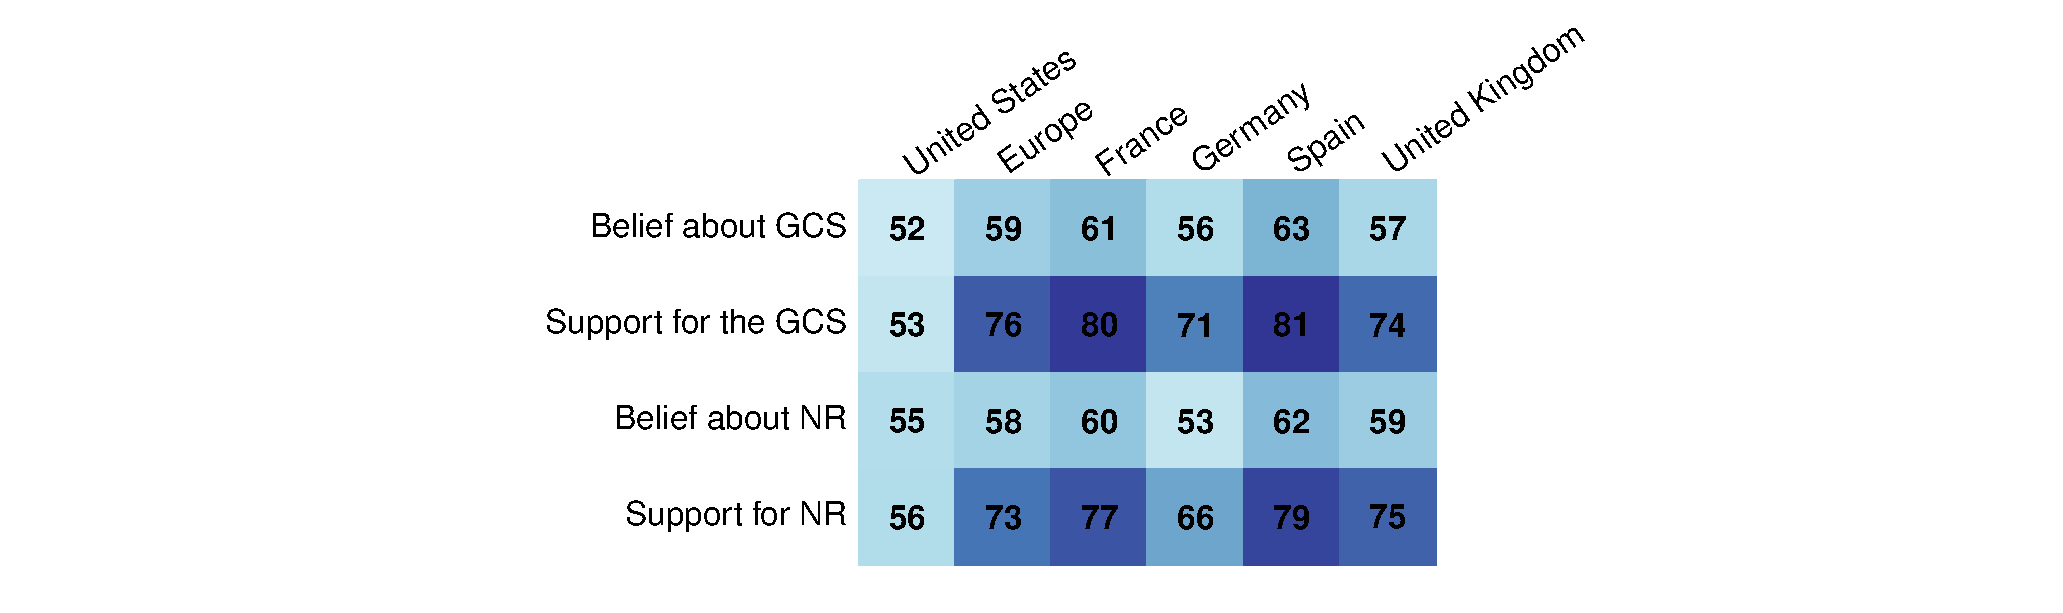
\includegraphics[width=.7\textwidth]{../figures/country_comparison/belief_all_mean.pdf}} 
% \end{figure}

\subsection{Stated support for global redistribution}\label{subsec:support_other}

\subsubsection{Global wealth tax}\label{subsubsec:support_global_wealth_tax}
%\paragraph{Global wealth tax}

Consistent with the results of the Global survey, a ``tax on millionaires of all countries to finance low-income countries'' garners relative support of over 69\% in each country, only 5 p.p. lower than a national millionaires tax overall (Figure \ref{fig:support}). In random subsamples, we inquire about respondents' preferences regarding the redistribution of revenues from a global tax on individual wealth exceeding \$5 million, after providing information on the revenue raised by such a tax in their country compared to low-income countries. 
% \footnote{A 2\% tax on net wealth exceeding \$5 million would annually raise \$816 billion, leaving unaffected 99.9\% of the world population. More specifically, it would collect \euro{}5 billion in Spain, \euro{}16 billion in France, £20 billion in the UK, \euro{}44 billion in Germany, \$430 billion in the U.S., and \$1 billion collectively in all low-income countries (28 countries, home to 700 million people).%Figures come from \citet{chancel_world_2022}, the \href{https://wid.world/world-wealth-tax-simulator/}{WID wealth tax simulator}, and the World Bank. % TODO: do they?
% } 
We ask certain respondents ($n$ = 1,283) what percentage of global tax revenues should be pooled to finance low-income countries. In each country, at least 88\% of respondents indicate a positive amount, with an average of one-third %ranging from 30\% (Germany) to 36\% (U.S., France) 
(Figure \ref{fig:global_share_mean}). To other respondents ($n$ = 1,233), we inquire whether they would prefer each country to retain all the revenues it collects or that half of the revenues be pooled to finance low-income countries. Approximately half of the respondents opt to allocate half of the tax revenues to low-income countries, consistently with the other variant of the question.

% \begin{figure}
%     \centering 
%     \caption[Preferred share of wealth tax for low-income countries]{[For Supplementary Material] Percent of global wealth tax that should finance low-income countries (\textit{mean}). \\ ``Imagine a wealth tax on households with net worth above [\$]5 million, enacted in all countries around the world.  
%     (\dots)  \\
%     What percentage should be pooled to finance low-income countries (instead of retained in the country's national budget)?'' (Question \ref{q:global_tax_global_share})} % TODO? n
%     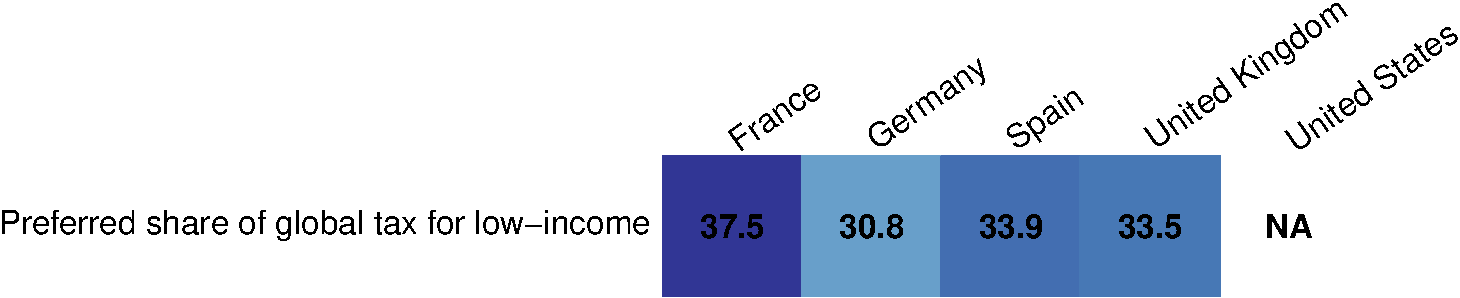
\includegraphics[width=1\textwidth]{../figures/country_comparison/global_tax_global_share_mean.pdf} \label{fig:global_share_mean}
% \end{figure}


\subsubsection{Other global policies}\label{subsubsec:support_other_global_policies} % NCCcomment
%\paragraph{Other global policies}

We also assess support for other global policies (Figure \ref{fig:support}). Most policies garner relative majority support in each country, with two exceptions: the ``cancellation of low-income countries' public debt'' and ``a maximum wealth limit'' for each individual. % In US pilot (n=86), 36% relative support to cap wealth at 100M (67% in Eu)
The latter policy obtains relative majority support in Europe but not in the U.S., despite the cap being set at \$10 billion in the U.S. compared to \euro{}/£100 million in Europe. Notably, climate-related policies enjoy significant popularity, with ``high-income countries funding renewable energy in low-income countries'' receiving absolute majority support across all surveyed countries. Additionally, relative support for loss and damages compensation, as approved in principle at the international climate negotiations in 2022 (``COP27''), ranges from 55\% (U.S.) to 81\% (Spain). %, with absolute support ranging from 41\% to 62\%.

% \setcounter{figure}{2}
% \renewcommand{\thefigure}{\arabic{figure}}
\begin{figure}
  % MAJOR figure
  \caption[Relative support for other global policies]{Relative support for various global policies (percentage of \textit{somewhat} or \textit{strong support}, after excluding \textit{indifferent} answers). (Questions \ref{q:climate_policies} and \ref{q:other_policies}; See Figure \ref{fig:support_likert_positive} for the absolute support.)% $n_\text{US} = n_\text{Eu} = 3,000,\, n_\text{FR} = 729,\, n_\text{DE} = 929,\, n_\text{ES} = 543,\, n_\text{UK} = 749, n_\text{US, global/national wealth tax} = 2,000$
  }
  \makebox[\textwidth][c]{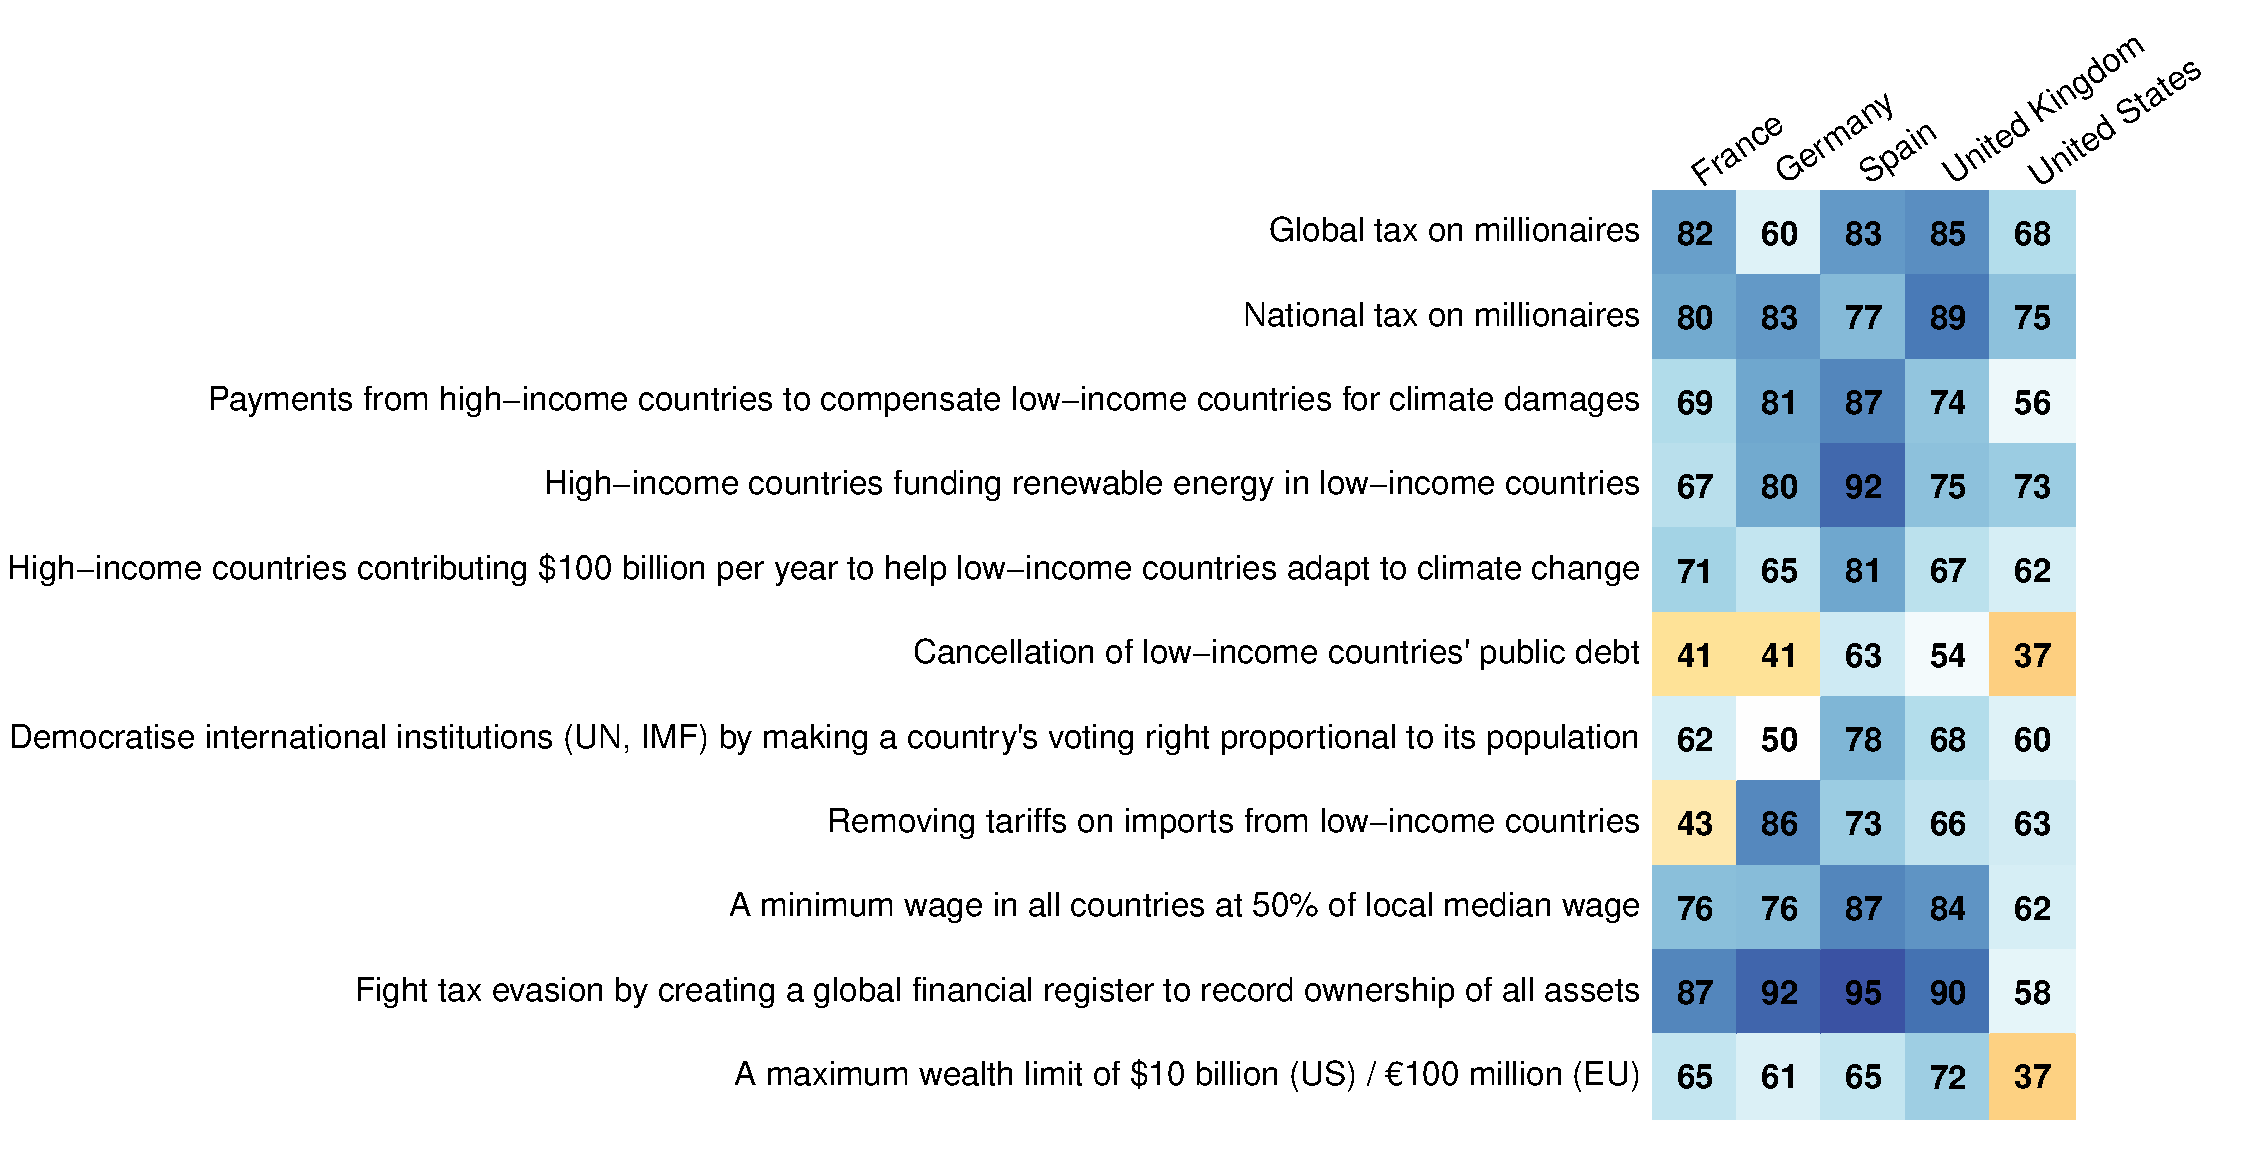
\includegraphics[width=\textwidth]{../figures/country_comparison/support_likert_share.pdf}}\label{fig:support}
\end{figure} 
% \setcounter{figure}{5}
% \renewcommand{\thefigure}{S\arabic{figure}}

\subsubsection{Foreign aid}\label{subsubsec:support_foreign_aid} % NCCcomment
%\paragraph{Foreign aid}

We provide respondents with information about the actual amount ``spent on foreign aid to reduce poverty in low-income countries'' relative to their country's government spending and GDP. Less than 16\% of respondents state that their country's foreign aid should be reduced, while 62\% express support for increasing it, including 17\% who support an unconditional increase (Figure \ref{fig:foreign_aid_raise_support}). Among the 45\% who think aid should be increased under certain conditions, we subsequently ask them to specify the conditions they deem necessary (Figure \ref{fig:foreign_aid_condition}). The three most commonly selected conditions are: ``we can be sure the aid reaches people in need and money is not diverted'' (73\% chose this condition), ``that recipient countries comply with climate targets and human rights'' (67\%), and ``that other high-income countries also increase their foreign aid'' (48\%). %\footnote{It is worth noting that these conditions align closely with the principles of the GCS.} 
On the other hand, respondents who do not wish to increase their country's foreign aid primarily justify their view by prioritizing the well-being of their fellow citizens or by perceiving each country as responsible for its own fate (Figure \ref{fig:foreign_aid_no}). In response to an open-ended question regarding measures high-income countries should take to fight extreme poverty, a large majority of Americans expressed that more help is needed (Figure \ref{fig:poverty_field}). The most commonly suggested form of aid is financial support, closely followed by investments in education. 


We also inquire about the perceived amount of foreign aid. Consistent with prior research (see Appendix \ref{subsubsec:literature_foreign_aid}), most people overestimate the actual amount of foreign aid (Figure \ref{fig:foreign_aid_belief}). We then elicit respondents' preferred amount of foreign aid, after randomly presenting them with either the actual amount or no information. Most of the respondents who learn the actual amount choose a bracket at least as high as the actual one, and most of those without the information choose a bracket at least as high as the perceived one (Figures \ref{fig:foreign_aid_amount}--\ref{fig:foreign_aid_preferred_info}). Finally, we ask a last question to the respondents who received the information. To those who prefer an increase of foreign aid, we ask how they would finance it: by far, the preferred source of funding is higher taxes on the wealthiest (Figure \ref{fig:foreign_aid_raise_how}). To those who prefer a reduction, we ask how they would use the funds becoming available: %resulting savings: 
In every country, more people choose higher spending on education or healthcare rather than lower taxes (Figure \ref{fig:foreign_aid_reduce_how}). 


\begin{tcolorbox}\label{subsec:universalistic}
  \paragraph{Universalistic values}
% \subsection{Universalistic values}\label{subsec:universalistic}
% H4: A strong majority is universalist/cosmopolitan (TODO: which word?), even a majority for non-Republican
% TD It is not obvious how these answers are informative of malleable opinions. So I don't think we should state the hypothesis and sell this as a test.
%Another hypothesis to explain the discrepancy between the lack of interest for global policies in the public debate despite a strong stated support is that opinions on the topic are weak and malleable. A way to test this is to

We elicit underlying values, to test whether broad values are consistent with people's support for specific policies. %To better understand people's support for specific policies, we also ask broad questions to study their values. %We ask broad questions on people's values to see whether their core values are consistent with universalism. 
% We also elicit underlying values, to test whether values are consistent with people's support for specific policies. Most people express some degree of universalism, consistently with the support for specific policies. 
When we ask respondents which group they defend when they vote, % ($n$ = 6,000)
20\% choose ``sentient beings (humans and animals),'' 22\% choose ``humans,'' 33\% select their ``fellow citizens'' (or ``Europeans''), 15\% choose ``My family and myself,'' and the remaining 10\% choose another group (mainly ``My State or region'' or ``People sharing my culture or religion''). 
% The first two categories, representing close to one out of two people, 
% can be described as universalist in their vote. 
Notably, a majority of left-wing voters choose \textit{humans} or \textit{sentient beings}. 
% are universalist in their vote (see Figure \ref{fig:main_by_vote}). % for main attitudes by vote).% The share of universalist even constitutes a majority of left-wing voters

%Regarding the priorities of their country's diplomats in international climate negotiations, 
When asked what their country's diplomats should defend in international climate negotiations, only 11\% prefer their country's ``interests, even if it goes against global justice.'' In contrast, 30\% prefer global justice (with or without consideration of national interests), and the bulk of respondents (38\%) prefer their country's ``interests, to the extent it respects global justice.''

Furthermore, when we ask respondents to assess the extent to which climate change, global poverty, and inequality in their country are issues, climate change is generally viewed as the most significant problem % , followed by global poverty and national inequality.
(with a mean score of 0.59 after recoding answers between -2 and 2). This is followed by global poverty (0.42) and national inequality (0.37). %, $n$ = 6,000).

Finally, we conduct a lottery experiment to elicit. % universalistic values. 
Respondents were automatically enrolled in a lottery with a \$100 prize and had to choose the proportion of the prize they would keep for themselves versus give to a person living in poverty. The % Finally, we created a lottery, where respondents choose the proportion of the \$100 prize they would keep for themselves versus give to a person living in poverty. The 
charity donation is directed either to an African individual or a fellow citizen, depending on the respondent's random assignment. In Europe, we observe no significant variation in the willingness to donate based on the recipient's origin. In the U.S., the donations to Africans are 3 p.p. lower, %(with an average donation of 34\%), 
but the slightly lower donations to Africans are entirely driven by Trump voters and non-voters (Table \ref{tab:donation}).

% TODO! put back?
% Overall, answers to these broad value questions are consistent with half of Americans and three quarters of Europeans supporting global policies like the GCS: people are almost as much willing to give to poor Africans than to poor fellow citizens, find that global issues are among the biggest problems, almost half of them are universalist when they vote, and most of them wish that their diplomats take into account global justice.
\end{tcolorbox}

% \begin{figure}[h!]
%   \caption[Attitudes on the evolution of foreign aid]{[For Supplementary Material] Attitudes regarding the evolution of [own country] foreign aid. (Question \ref{q:foreign_aid_raise_support})}\label{fig:foreign_aid_raise_support}
%   \makebox[\textwidth][c]{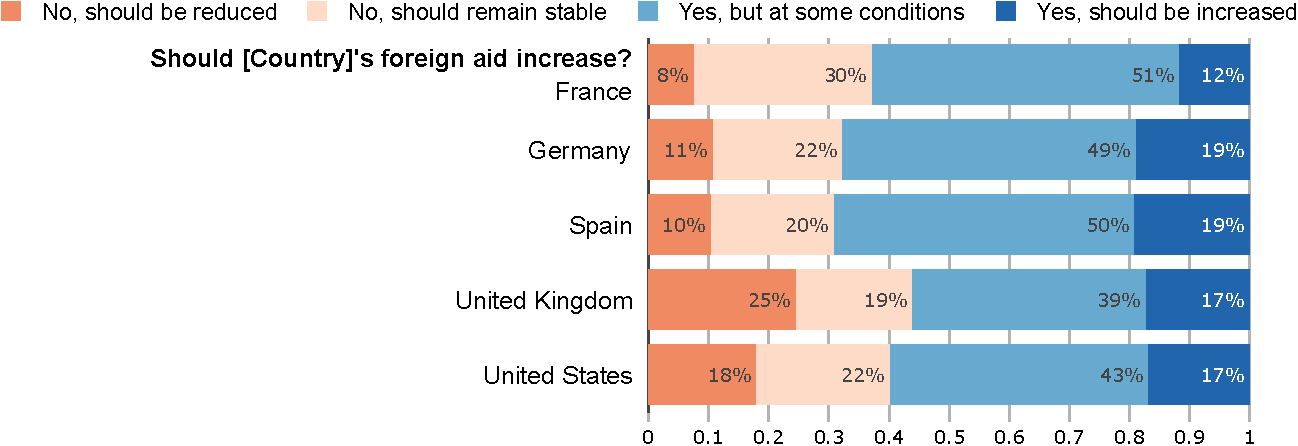
\includegraphics[width=\textwidth]{../figures/country_comparison/foreign_aid_raise_support.pdf}} 
% \end{figure}

% \begin{figure}[h!]
%   \caption[Conditions at which foreign aid should be increased]{[For Supplementary Material] Conditions at which foreign aid should be increased (in percent). [Asked to those who wish an increase of foreign aid at some conditions.] (Question \ref{q:foreign_aid_condition})}\label{fig:foreign_aid_condition}
%   \makebox[\textwidth][c]{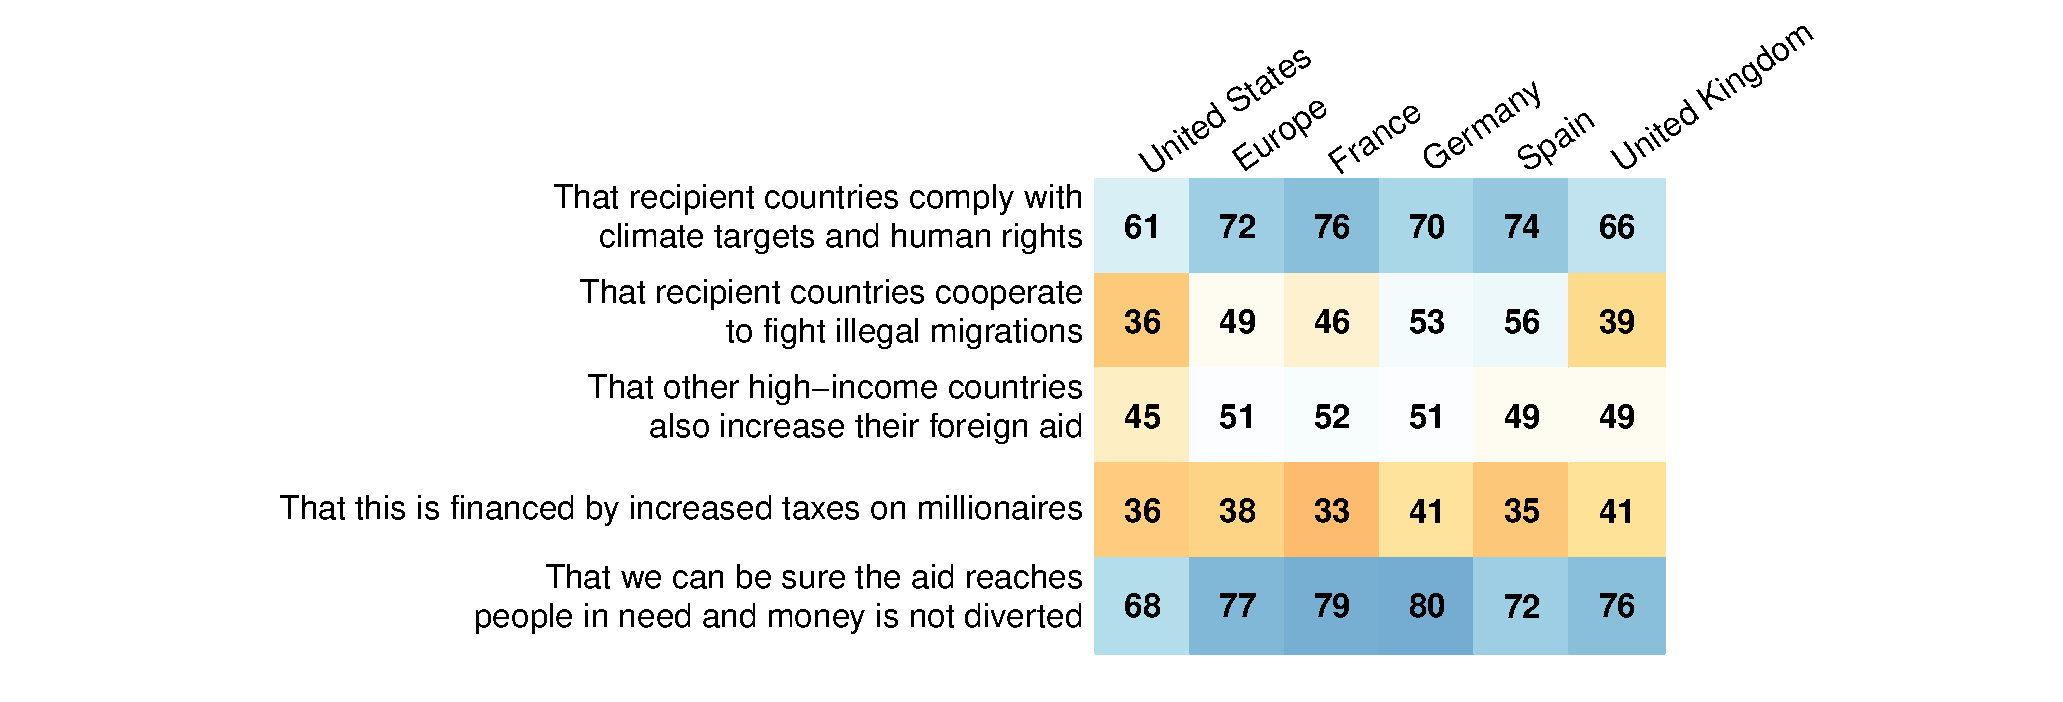
\includegraphics[width=\textwidth]{../figures/country_comparison/foreign_aid_condition_positive.pdf}} 
% \end{figure}

% \begin{figure}[h!]
%   \caption[Reasons why foreign aid should not be increased]{[For Supplementary Material] Reasons why foreign aid should not be increased (in percent). [Asked to those who wish a decrease or stability of foreign aid.] (Question \ref{q:foreign_aid_no})}\label{fig:foreign_aid_no}
%   \makebox[\textwidth][c]{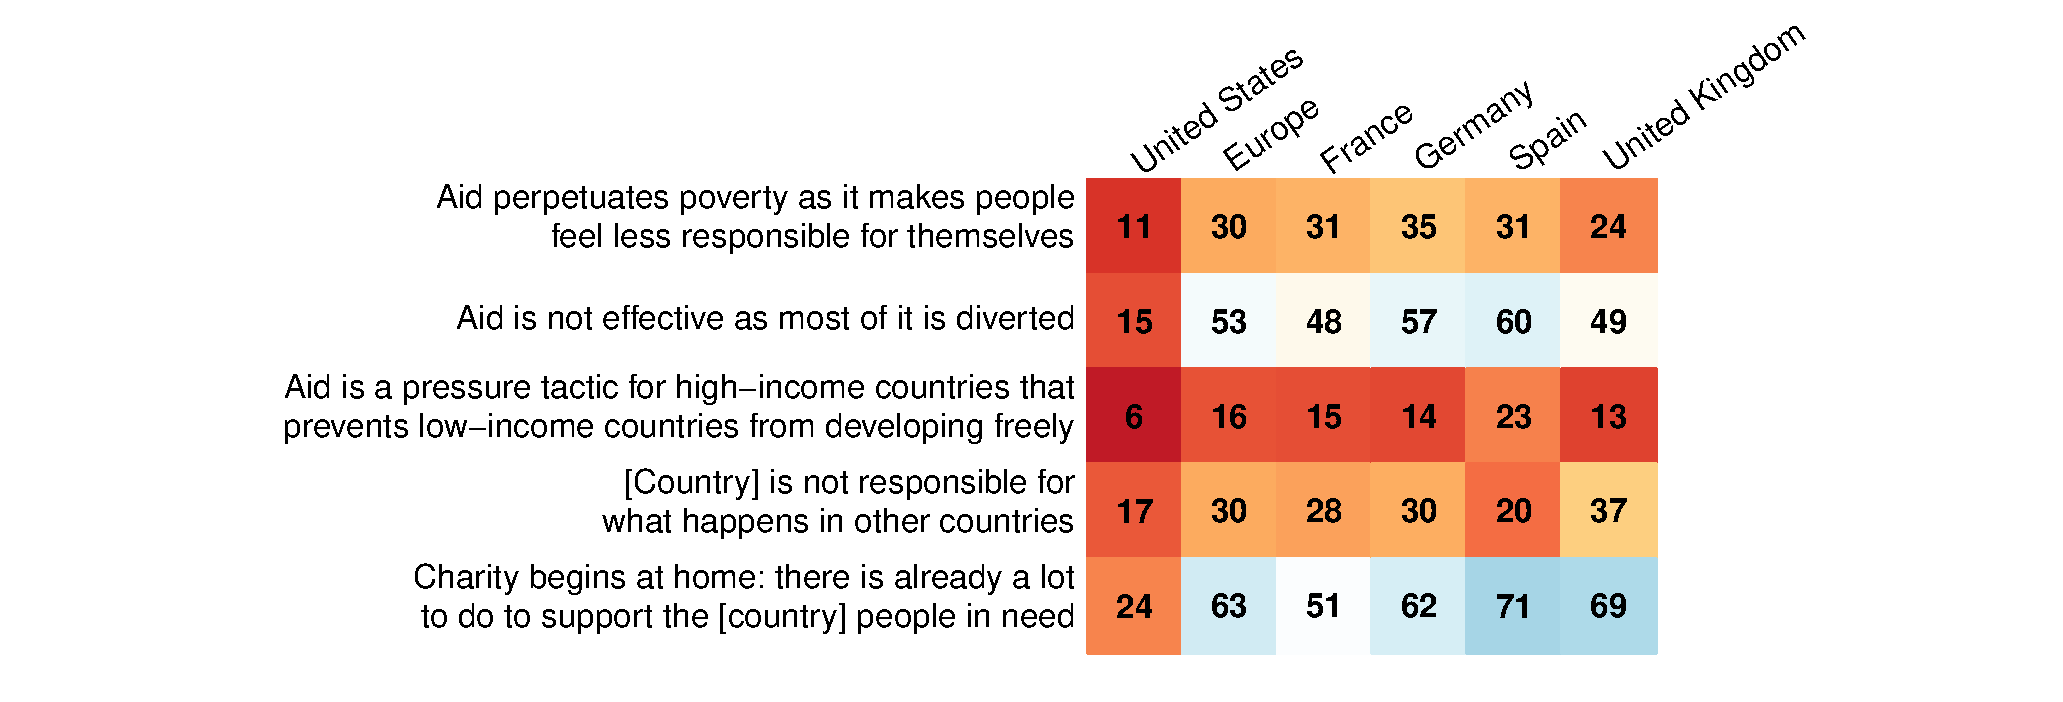
\includegraphics[width=\textwidth]{../figures/country_comparison/foreign_aid_no_positive.pdf}} 
% \end{figure}

\section{Discussion} % Summary, conclusion

% TODO! The discussion section must include a transparent discussion of limitations

% TODO? give less space to OECD paper?
Our point of departure are recent surveys conducted %by \citet{dechezlepretre_fighting_nodate} 
in 20 of the largest countries% \citep{dechezlepretre_fighting_nodate}
, as they reveal strong majority support for global redistributive and climate policies, even in high-income countries that would financially lose from them. The results from the Main surveys conducted in the U.S. and four European countries %presented here 
reinforce these findings. We find strong support for global taxes on the wealthiest individuals, as well as majority support for our main policy of interest -- the Global Climate Scheme (GCS). The GCS encompasses carbon pricing at a global level through an emissions trading system, accompanied by a global basic income funded by the scheme's revenues. Additional experiments, such as a list experiment and a real-stake petition, demonstrate that the support for the GCS is real. 
Such genuine support is further substantiated by the prioritization of the GCS over prominent national climate policies and aligned with a significant portion of the population holding universalistic values rather than nationalistic or egoistic ones. Moreover, the conjoint analyses indicate that a progressive candidate would not lose voting shares by endorsing the GCS, and may even gain 11 p.p. in voting shares in France. Similarly, a candidate endorsing the GCS would gain votes in a U.S. Democratic primary, while in Europe, a progressive platform that includes the GCS would be preferred over one that does not.

Having ruled out insincerity %and underestimation of fellow citizens' support 
as potential explanation for the scarcity of global policies in the public debate, we propose alternative explanations. %As we ruled out all hypotheses of our registration plan,\footnote{The project was preregistered in the Open Science Foundation registry (\href{https://osf.io/fy6gd}{osf.io/fy6gd}).} we now need to study new explanations.
The first two are variations of pluralistic ignorance, and the last three represent complementary explanations. 

First, there may be pluralistic ignorance \textit{among policymakers} regarding universalistic values, support for the GCS, or the electoral advantage of endorsing it. Second, people or policymakers may believe that globally redistributive policies are politically infeasible in some key (potentially foreign) countries like the U.S. % We intend to test these hypotheses by running a survey on Congress staffers and Members of the European Parliament.  %Second, there may be a more subtle form of pluralistic ignorance: although most people correctly predict what people would answer to a survey question, they may view globally redistributive policies as unrealistic, perhaps because they have never reflected upon the fact that many people across the world hold univeralistic values and are supportive of global solidarity. Third, most people and perhaps even most policy makers may have simply never heard of the GCS, let alone built their political ideas upon it. 
Third, political discourse centrally happens at the national level, shaped by national media and institutions such as voting. 
National framing by political voices may create biases and suppress universalistic values. % Third, most institutions are national: the largest scale votes take place at the national level% so political platforms are devised at this level, most media target a national audience, most commentators frame their discourse from a national perspective and portray relations to foreign countries as conflictual. 
Fourth, many individuals, including policymakers, may perceive global redistributive policies as ill-defined or technically infeasible, ultimately dismissing them as unrealistic. In particular, policymakers may have insider information about the technical feasibility of such policies. Alternatively, the perception of unrealism may stem from an unawareness of specific proposals. % cautiously doubt that they are well-specified
% TODO? rewrite as a fifth hypothesis that the policies may indeed not be well specified nor implementable?
% Fourth, many individuals, including policymakers, may simply be unaware of specific global redistributive policies, let alone base their political ideas on them. This lack of awareness may lead people to % cautiously doubt that they are well-specified
% perceive such policies as ill-defined or technically infeasible, ultimately dismissing them as unrealistic. % TODO? rewrite as a fifth hypothesis that the policies may indeed not be well specified nor implementable?
% The latter hypothesis is supported by the prior ignorance of the GCS expressed in the feedback fields, where a common response is a variation of ``thank you for this interesting, thought-provoking survey.'' 
% TODO? remove?
Fifth, just as policy is disproportionately influenced by the economic elites,\citep{gilens_testing_2014,persson_rich_2023} public debate may be shaped by the wealthiest, who have vested interests in preventing global redistribution.

% Also: vested interest influence on elites (a la Gilens and Page for the US, Persson & Sundell 23), cf. Boone story
% decline of support the more specific a measure gets / enters the public debate => addressed in conclusion of pros and cons
% people not believing that the policy is technically implementable => addressed
% politicians seeing defects or lack of specification of the policy that warrant opposition, while ignorant citizens would naively like it => addressed
% platform don't matter for vote

% LM This are all legtimiate and important points. For a global transfer (rather than say a EU transfer), I am really missing remarks about (lack) of quality of governance, rent creation and capture, corruption etc. To play devil's advocate, as much as I am sympathetic to the idea, I'm not sure I would currently vote in favor of such policies. Why? Not because I dislike the idea, but I am not sure that my carbon tax rent as a German would actually reach the poor population of Indonesia or Nigeria rather than the pockets of cleptocratic elites :) I'd like the draft to reflect that and could make an attempt to pre-empt that objection based on some references later in the project.
%In any case, 

Confirmation of any of these hypotheses would lead to a common conclusion: there exists substantial support for global policies addressing climate change and global inequality, even in high-income countries, and the perceived boundaries of political realism on this issue may soon shift. %Recent developments suggest that such a change might be underway: the \citet{african_union_african_2023} calls for a global carbon taxation regime, a call quickly endorsed by the President of the EU Commission;\footnote{Cf. this tweet by Ursula von der Leyen: \href{https://twitter.com/vonderleyen/status/1700416700238225659}{twitter.com/vonderleyen/status/1700416700238225659}.} the \citet{un_promotion_2023} is setting up a Framework Convention on International Tax Cooperation, where various countries want to open discussions about a global wealth tax; Brazil uses its presidency of the G20 in 2024 to propose a global tax to finance sustainable development; the International Maritime Organization is poised to adopt a global carbon levy on maritime fuel; etc. 
Uncovering evidence to support the above hypotheses could %help
draw attention to global policies in the public debate and contribute to their increased prominence. % Uncovering evidence for this might actually contribute itself to garner more attention to global policies in the public debate. 

% Also: no short term outcome (before the end of the mandate) so no incentive to start it

% TODO!? alternative conclusion: strong and sincere support for global wealth tax in both continents => probable reason why it's not more discussed is that it's not the determining issue for voters. Strong and sincere support for the GCS in Europe but half-half in the U.S. (where there is a risk that support decreases in a campaign) => not endorsed by the Democrats because they seek policies more strongly supported, and not discussed in Europe probably because the U.S. won't support it.

% For warm glow and how to test it, see my 28/6, 30/6,  (2023) emails (elicit beliefs on feasibility/obstacles, ask support for Bridgetown / 100G€ with vs. without saying it may be approved at the COP, redo conjoint analysis without support question before, asking for approval of global redistr. policy costing 50€/month with/without asking for a similar one costing 20€/month before). 
% For new survey, also test one ambitious (no one with less than 7$/day), unilateral global wealth tax and GCP with partial participation
